% !TeX root = ./main.tex
%% Master Thesis Template
%% Please update the specification through this link: https://daim.idi.ntnu.no/howto_thesis_submission.pdf

\documentclass[pdftex,10pt,b5paper,twoside,openany]{book}
% \documentclass[pdftex,10pt,b5paper,twoside]{book}
\usepackage[lmargin=25mm,rmargin=25mm,tmargin=27mm,bmargin=30mm]{geometry}
\usepackage[titletoc]{appendix}
% !TeX root = main.tex
\usepackage[parfill]{parskip}
\usepackage{setspace}
\usepackage[export]{adjustbox}
\usepackage{graphicx}
\usepackage{amssymb}
\usepackage{mathrsfs}
\usepackage{amsthm}
\usepackage{mathtools}
\usepackage{amsmath}
\usepackage{color}
\usepackage{xargs}
\usepackage{mdframed} % Removed [framemethod=tikz]
\usepackage[most]{tcolorbox} % Add tcolorbox and breakable library
\tcbuselibrary{breakable} % Explicitly load breakable library
\usepackage{capt-of}
\usepackage{subcaption}
\usepackage[pdftex,dvipsnames]{xcolor}
\usepackage{transparent}
\usepackage{svg}
\usepackage{pythonhighlight}
\usepackage[colorinlistoftodos,prependcaption,textsize=small]{todonotes}
\usepackage[Lenny]{fncychap}
\usepackage[pdftex,bookmarks=true]{hyperref}
\usepackage[pdftex]{hyperref}
\hypersetup{
    colorlinks,%
    citecolor=black,%
    filecolor=black,%
    linkcolor=black,%
    urlcolor=black
}
\usepackage[capitalize]{cleveref}
\crefname{equation}{}{}
\Crefname{equation}{Equation}{}
\crefname{figure}{Figure}{figures}
\crefname{section}{Section}{sections}
\usepackage[font=small,labelfont=bf]{caption}
\usepackage{fancyhdr}
\usepackage{times}
%\usepackage[intoc]{nomencl}
%\renewcommand{\nomname}{List of Abbreviations}
%\makenomenclature
\usepackage{natbib}
\usepackage[style=altsuper4col,acronym]{glossaries}
% \usepackage[style=altsuper4colheader]{glossaries}
\usepackage{float}
\usepackage{flafter} 
\usepackage[section]{placeins} % Prevent floats from floating into the next section - Relaxed options
%\floatstyle{boxed} 

% ShareLaTeX does not support glossaries now. Sorry...
%\usepackage[number=none]{glossary}
%\makeglossary
%\newglossarytype[abr]{abbr}{abt}{abl}
%\newglossarytype[alg]{acronyms}{acr}{acn}
%\newcommand{\abbrname}{Abbreviations} 
%\newcommand{\shortabbrname}{Abbreviations}
%%\makeabbr
\newcommand{\HRule}{\rule{\linewidth}{0.5mm}}

\renewcommand*\contentsname{Table of Contents}

\pagestyle{fancy}
\fancyhf{}
\renewcommand{\chaptermark}[1]{\markboth{\chaptername\ \thechapter.\ #1}{}}
\renewcommand{\sectionmark}[1]{\markright{\thesection\ #1}}
\renewcommand{\headrulewidth}{0.1ex}
\renewcommand{\footrulewidth}{0.1ex}
\fancypagestyle{plain}{\fancyhf{}\fancyfoot[LE,RO]{\thepage}\renewcommand{\headrulewidth}{0ex}}

\makeglossaries

\DeclareMathOperator{\asin}{asin}
\DeclareMathOperator{\acos}{acos}
\DeclareMathOperator{\atan}{atan}
\DeclareMathOperator{\sign}{sign}
\DeclareMathOperator*{\argmin}{arg\,min}
\DeclareMathOperator{\unique}{unique}

\newcommandx{\unsure}[2][1=]{\todo[linecolor=red,backgroundcolor=red!25,
bordercolor=red,#1]{#2}} \newcommandx{\change}[2][1=]{\todo[linecolor=blue,
backgroundcolor=blue!25,bordercolor=blue,#1]{#2}}
\newcommandx{\info}[2][1=]{\todo[linecolor=OliveGreen,backgroundcolor=OliveGreen!
25,bordercolor=OliveGreen,#1]{#2}}
\newcommandx{\improvement}[2][1=]{\todo[linecolor=Plum,backgroundcolor=Plum!25,
bordercolor=Plum,#1]{#2}} 
\newcommandx{\emil}[2][1=]{\todo[linecolor=LimeGreen,backgroundcolor=LimeGreen!25,
bordercolor=LimeGreen,#1]{#2}}
\newcommandx{\morten}[2][1=]{\todo[linecolor=ForestGreen,backgroundcolor=ForestGreen!25,
bordercolor=ForestGreen,#1]{#2}}


%% Algorithm
\usepackage[T1]{fontenc}
\usepackage[utf8]{inputenc} % set input encoding
\usepackage{varwidth}

\usepackage{newfloat}
\DeclareFloatingEnvironment[placement=htp]{algorithm}
\usepackage{algpseudocodex}

\usepackage{caption}
\let\globalcaption=\caption
\usepackage{setspace}

% Change caption format
\captionsetup[algorithm]{
    belowskip=0pt,
    aboveskip=0pt,
    % font=scriptsize,
    justification = raggedright,
    singlelinecheck = false,
    name = Algorithm
}

% Change width of horizontal lines 
\makeatletter
\newcommand{\algrule}[1][1pt]{\par\vskip.5\baselineskip\hrule height#1\vskip.5\baselineskip}
\makeatother



% Add numbered property environment
\newtheorem{property}{Property}
\crefname{property}{Property}{properties}

% Add numbered example environment with standout style and indented
\theoremstyle{definition}
\newtheorem{example}{Example}[chapter]
\crefname{example}{Example}{examples}

\newenvironment{indentedexample}[1][]
    {\par\begin{example}[#1]
        \begin{mdframed}[
            linewidth=1pt,
            linecolor=black,
            bottomline=false,topline=false,rightline=false,
            innerrightmargin=0pt,innertopmargin=0pt,innerbottommargin=0pt,
            innerleftmargin=1em,% Distance between vertical rule & proof content
            skipabove=1\baselineskip % Keep space above relative to title
            % Removed skipbelow
            ]}
{\end{mdframed}\vspace{\baselineskip}\end{example}} % Add vspace after mdframed
    
% Add numbered math algorithm environment
\newtheorem{mathalgo}{Algorithm}[chapter]
\crefname{mathalgo}{Algorithm}{algorithms}

% Def eq command
\newcommand{\defeq}{\vcentcolon=}
\newacronym{VO}{VO}{Velocity Obstacle}
\newacronym{COLREGS-VO}{COLREGS-VO}{COLREGS-compliant Velocity Obstacle}
\newacronym{COLREGS}{COLREGS}{Convention on the International Regulations for Preventing Collisions at Sea}
\newacronym{MPC}{MPC}{Model Predictive Control}
\newacronym{NMPC}{NMPC}{Nonlinear Model Predictive Control}
\newacronym{V2V}{V2V}{Vessel to Vessel Encounter}
\newacronym{LOS}{LOS}{Line of Sight}
\newacronym{OS}{OS}{Own Ship}
\newacronym{TS}{TS}{Target Ship}
\newacronym{CPA}{CPA}{Closest Point of Approach}
\newacronym{TCPA}{TCPA}{Time to Closest Point of Approach}
\newacronym{MIQP}{MIQP}{Mixed Integer Quadratic Programming}
\newacronym{MIQCP}{MIQCP}{Mixed Integer Quadratically Constrained Programming}
\newacronym{MILP}{MILP}{Mixed Integer Linear Programming}
\newacronym{MISOCP}{MISOCP}{Mixed Integer Second Order Cone Programming}
\newacronym{MISDP}{MISDP}{Mixed Integer Semidefinite Programming}
\newacronym{MINLP}{MINLP}{Mixed Integer Nonlinear Programming}
\newacronym{MIP}{MIP}{Mixed Integer Programming}
\newacronym{SOCP}{SOCP}{Second Order Cone Programming}
\newacronym{SDP}{SDP}{Semidefinite Programming}
\newacronym{NLP}{NLP}{Nonlinear Programming}
\newacronym{LP}{LP}{Linear Programming}
\newacronym{QP}{QP}{Quadratic Programming}
\newacronym{SOS1}{SOS1}{Special Ordered Set of type 1}
\newacronym{SOS2}{SOS2}{Special Ordered Set of type 2}
\newacronym{OCP}{OCP}{Optimal Control Problem}
\newacronym{XTE}{XTE}{Cross Track Error}
\newacronym{ATE}{ATE}{Along Track Error} 
\newacronym{TTE}{TTE}{Total Track Error}
\newacronym{PMS}{PMS}{Preferred Maneuver Side}
\newacronym{CMS}{CMS}{Chosen Maneuver Side}
\newacronym{NURBS}{NURBS}{Non-Uniform Rational B-Spline}
\newacronym{NED}{NED}{North-East-Down}

\begin{document}

%% PART 1
%%The title page will be automatically generated and added by the DAIM system
% % !TEX root = main.tex

\begin{titlepage}
    \begin{center}
        \vspace*{1cm}
        \algrule
        \huge
        MPC-based COLREGS-aware trajectory planning for surface vessels using B-splines and mixed integer optimization
        \algrule
        \LARGE
        Master's Thesis
        \vspace{1.5cm}

        
        \large
        Eirik Kolås

        \vspace{0.2cm}

        June 2025

        \vspace{0.8cm}

        
        \vfill
        
        \vspace{0.8cm}
        
        \includesvg[width=0.4\textwidth]{fig/illustrations/NTNU Kyb.svg}
        
        
    \end{center}
\end{titlepage}

\cleardoublepage
% !TEX root = main.tex

\section*{Preface}
\addcontentsline{toc}{chapter}{Preface}	



\cleardoublepage		%% Optional

%% PART 2
% !TeX root = main.tex
\pagenumbering{roman} 				
% \setcounter{page}{1}

\pagestyle{fancy}
\fancyhf{}
\renewcommand{\chaptermark}[1]{\markboth{\chaptername\ \thechapter.\ #1}{}}
\renewcommand{\sectionmark}[1]{\markright{\thesection\ #1}}
\renewcommand{\headrulewidth}{0.1ex}
\renewcommand{\footrulewidth}{0.1ex}
\fancyfoot[LE,RO]{\thepage}
\fancypagestyle{plain}{\fancyhf{}\fancyfoot[LE,RO]{\thepage}\renewcommand{\headrulewidth}{0ex}}

\section*{\large Abstract}
\addcontentsline{toc}{chapter}{Abstract}	
\vspace{0.5cm}


Safe navigation of autonomous surface vessels in crowded waterways demands strict adherence to the international regulations for preventing collisions at sea (COLREGS). 
This paper presents a novel mixed‐integer nonlinear model‐predictive control framework that leverages B‐spline trajectory parameterizations for both vessel states and time. It transforms kinematic, dynamic, and COLREGS constraints into convex or polynomial inequalities on the spline control‐point coefficients.
The method introduces a projected tracking error (PXTE) as an alternative to traditional cross-track error, improving alignment with spline-based references. A theoretical derivation also reveals that spline-based trajectory formulations inherently induce transient deceleration near inflection points, adding analytical insight into the structural consequences of the chosen  representation.
A Big–M mixed-integer scheme encodes port/starboard passage decisions via separating hyperplanes, enabling efficient resolution of the nonconvex collision-avoidance problem in a single mixed-integer nonlinear program (MINLP).
A novel inverse-Gramian weighting suppresses high-frequency oscillations in the tracking error without affecting maneuverability or requiring additional tuning. The resulting optimization problem is a sparse MINLP with gauranteed continuous-time constraint adherence that can be efficiently solved using a standard MINLP solver.

The method is implemented in Python with CasADi offering modular components for own-ship dynamics, obstacle models, and structured cost functions, made available as an open source library. Simulation scenarios---including stationary obstacles, head-on encounters, crossing situations, and overtaking maneuvers---demonstrate strict adhearance to collision avoidance constraints, and highly customizable trajectory shaping through simple spline weights on the different objective function terms. The results demonstrate that the proposed method can produce smooth and interpretable 
trajectories in complex scenarios, with structural insights into the spline-based formulation.

\cleardoublepage

\section*{Sammendrag}
\addcontentsline{toc}{chapter}{Sammendrag}
\vspace{0.5cm}

Trygg navigasjon i travle farvann krever streng etterlevelse av de internasjonale reglene for å forhindre sammenstøt til sjøs (COLREGS).
Denne artikkelen presenterer et rammeverk for modellprediktiv kontroll med blandet-heltallsprogrammering som benytter en B-spline-parametrisering av både fartøystsbaner og tid. Kinematiske, dynamiske og COLREGS-betingelser omformes til konvekse eller polynomielle ulikheter i spline-koeffisientene.
Metoden introduserer en projisert sporingsfeil (PXTE) som et alternativ til tradisjonell tverrsporingsfeil, noe som forbedrer samsvaret med spline-baserte referansebaner. En teoretisk utledning viser også at spline-baserte baneformuleringer iboende induserer transiente nedbremsinger nær infleksjonspunkter, noe som gir analytisk innsikt i de strukturelle konsekvensene av den valgte representasjonen.
En Big–M blandet-heltallsløsning koder beslutninger om babord/styrbord passering ved hjelp av separerende hyperplan, noe som muliggjør effektiv løsning av det ikke-konvekse kollisjonsunngåelsesproblemet i én enkelt blandet-heltalls ikkelineær program (MINLP).
En ny inverse-Gramian-vektlegging demper høyfrekvente svingninger i sporingsfeilen uten å redusere manøvrerbarhet eller kreve ekstra tuning. Det resulterende optimaliseringsproblemet er et glissent endelig-dimensjonalt MINLP med garantert kontinuerlig-tid overholdelse av beskrankningene som kan løses effektivt med en standard MINLP-løser.

Metoden er implementert i Python med CasADi og tilbyr modulære komponenter for egenfartøysdynamikk, modellering av hindringer og strukturerte kostnadsfunksjoner, tilgjengelig som et open source kode-bibliotek. Simuleringsscenarier — inkludert stasjonære hindringer, møte i motgående kurs, kryssende situasjoner og forbikjøringer — demonstrerer sømløs integrasjon av kontinuerlig-tid kollisjonsunngåelsesbegrensninger og justerbar baneform gjennom enkle spline-vekter på ulike ledd i objektivfunksjonen. Resultatene fremhever at metoden kan produsere robuste og jevne baner som fremmer COLREGS-etterlevelse i komplekse scenarier, med strukturelle innsikter i den spline-baserte formuleringen.

\cleardoublepage		%% Optional
% !TeX root = main.tex

\section*{Preface}
\addcontentsline{toc}{chapter}{Preface}
\vspace{0.5cm}


\begin{center}
    \vspace{1cm}
    Eirik Kolås\\
    Trondheim, June 20, 2024
\end{center}


\cleardoublepage		    %% Optional
\addcontentsline{toc}{chapter}{Table of Contents}
\tableofcontents
\clearpage

\listoffigures									
\addcontentsline{toc}{chapter}{List of Figures}
\clearpage

\listoftables
\addcontentsline{toc}{chapter}{List of Tables}
\clearpage
\listofalgorithms
\addcontentsline{toc}{chapter}{List of Algorithms}
			%% Generate TOC, list of tables, and list of figures automatically
% \renewcommand{\glossarysection}[2][]{
%    \section*{{\Huge Abbreviations}}
%    \addcontentsline{toc}{chapter}{Abbreviations}
%    \vspace{0.5cm}
% }
\glstoctrue
\printglossary[type=\acronymtype]
\printglossary[title=Glossary, toctitle=Glossary]


\cleardoublepage

\pagestyle{fancy}
\fancyhf{}
\renewcommand{\chaptermark}[1]{\markboth{\chaptername\ \thechapter.\ #1}{}}
\renewcommand{\sectionmark}[1]{\markright{\thesection\ #1}}
\renewcommand{\headrulewidth}{0.1ex}
\renewcommand{\footrulewidth}{0.1ex}
\fancyfoot[LE,RO]{\thepage}
\fancyhead[LE]{\leftmark}
\fancyhead[RO]{\rightmark}
\fancypagestyle{plain}{\fancyhf{}\fancyfoot[LE,RO]{\thepage}\renewcommand{\headrulewidth}{0ex}}

\pagenumbering{arabic} 				
\setcounter{page}{1}	%% Optional

%% PART 3 -- The Chapters
% !TeX root = main.tex
%===================================== CHAP 1 =================================

\chapter{Introduction}


\section{Motivation}

Rapid urbanization and the urgent need for sustainable transportation are driving cities to explore innovative mobility solutions. In particular, autonomous electric passenger increasingly gaining attention by cities as a sustainable mode of urban transit \citep{Alsos2024}. By leveraging existing waterways, such ferries can reduce reliance on carbon-intensive road vehicles and complement land-based public transport. 
This aligns with global sustainability objectives---addressing climate action goals and promoting sustainable cities and communities through zero-emission operations that mitigate greenhouse‐gas emissions and improve urban accessibility \citep{dnvAutonomousUrban}. 
As \citet{dnvAutonomousUrban} notes, autonomous electric ferries can meet transport needs with minimal environmental impact, help decongest traffic, and reduce the need for costly infrastructure such as new roads or bridges. This aligns with the United Nations Sustainable Development Goal 13 on climate action and SDG 11 on sustainable cities \citep{UN2024}.

Pioneering projects worldwide have demonstrated the feasibility of autonomous electric ferries. The milliAmpere2 ferry (shown in \cref{fig:intro-asv}), developed at NTNU in Trondheim, became the world’s first autonomous urban passenger ferry pilot open to the public in 2022, carrying over 1,500 passengers during a three‐week trial \citep{Alsos2024}. Building on these trials, commercial deployments have emerged: in 2023, an autonomous electric ferry service operated by Zeabuz entered Stockholm’s public transport network with their MF Estelle \citep{Alsos2024}. Similar initiatives include France’s Hyke prototype on the Seine and Amsterdam’s Roboat self‐navigating canal boats \citep{Alsos2024}. Development in this field is rapidly advancing, with research being conducted to address the challenges of human trust in autonomous systems, safety, situational awareness, and collision avoidance, to name a few \citep{Eide2025}.

\begin{figure}
    \centering
    \begin{subfigure}[t]{0.49\textwidth}
        \centering
        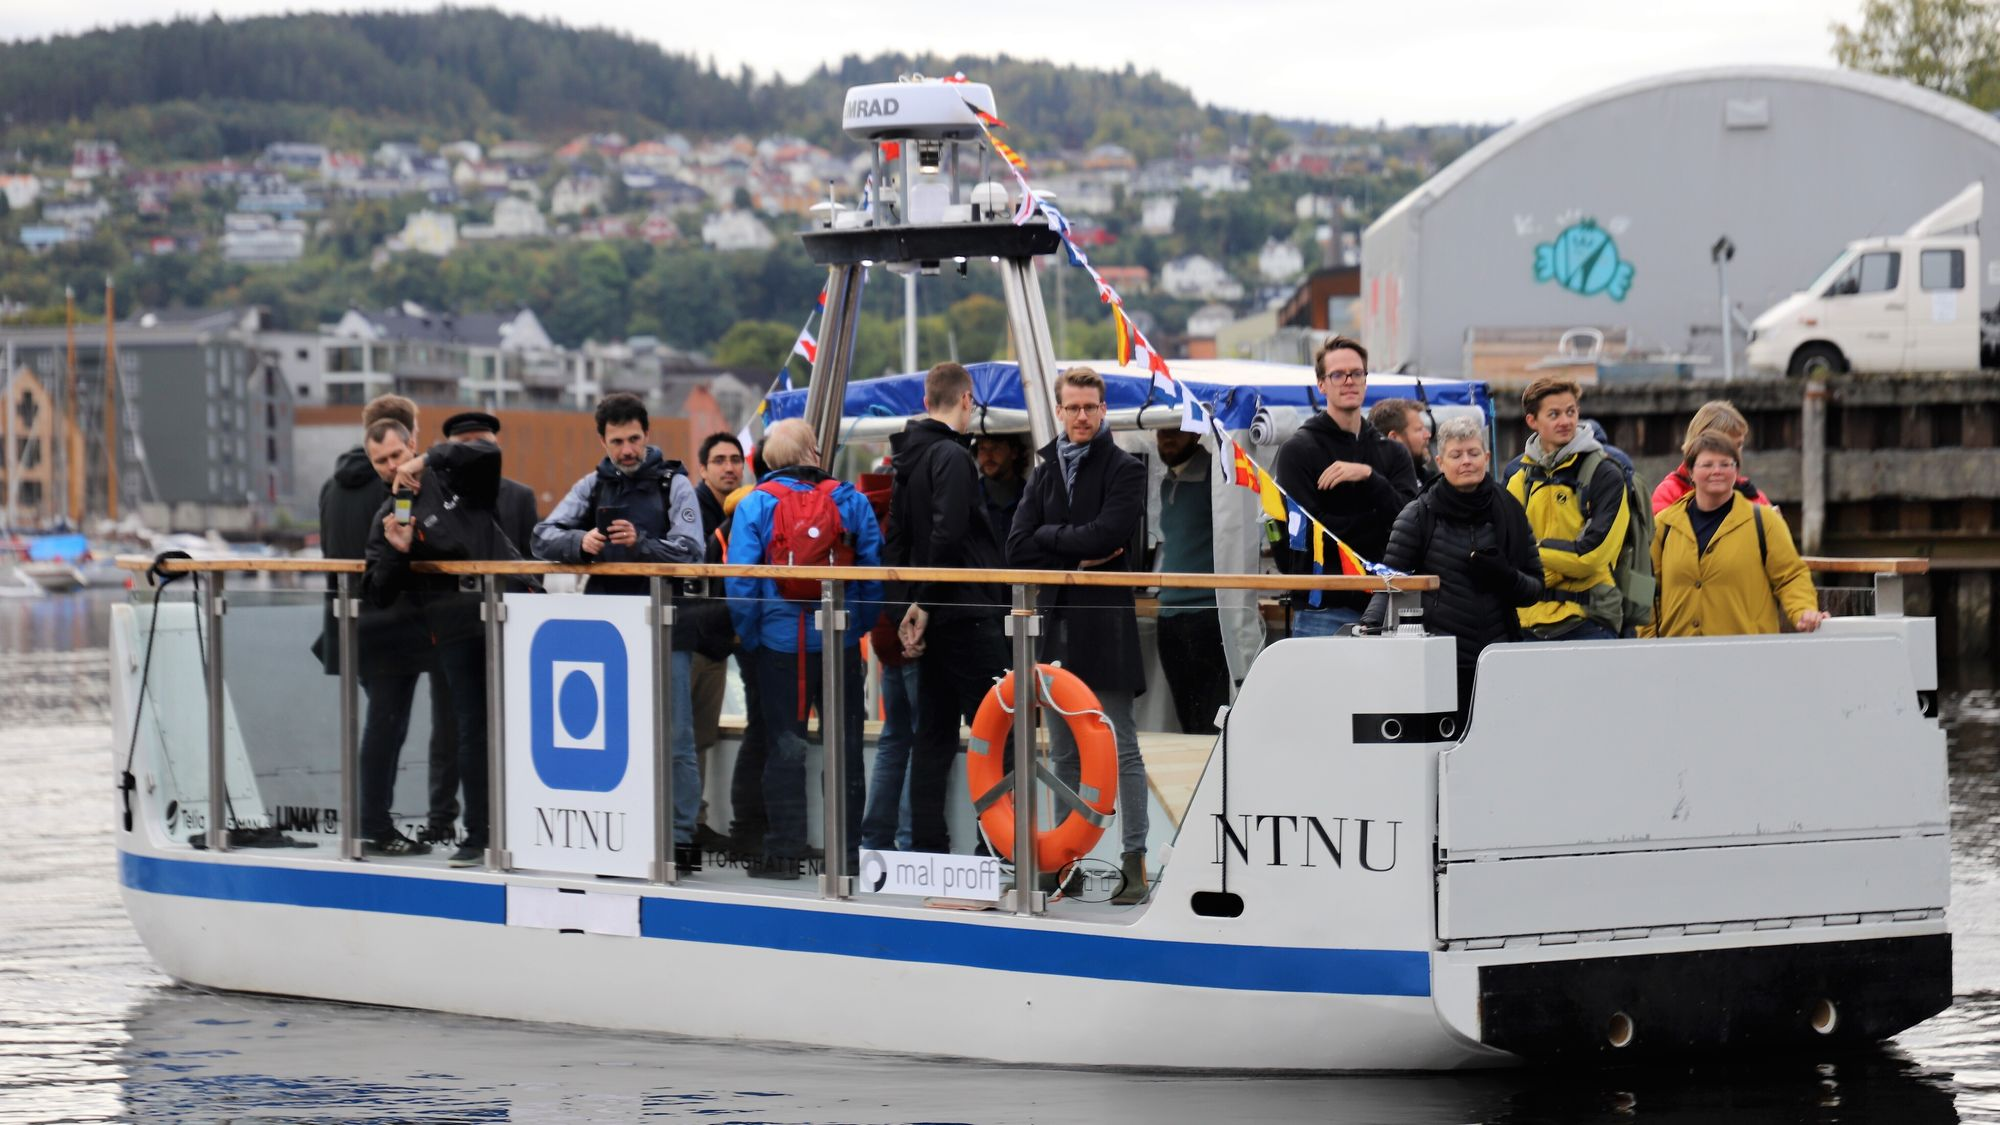
\includegraphics[width=\textwidth,height=100pt]{fig/images/milliampere.png}
        \caption{NTNU's ``milliAmpere2''. Image courtesy of \cite{tuFullTillit}.}
    \end{subfigure}%
    ~
    \begin{subfigure}[t]{0.49\textwidth}
        \centering
        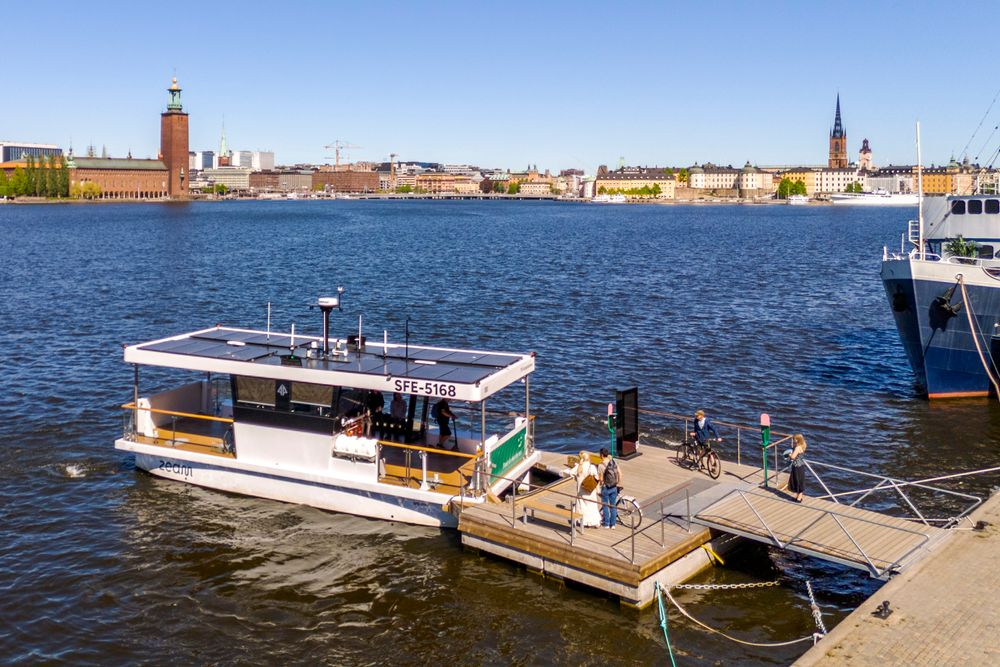
\includegraphics[width=\textwidth,height=100pt]{fig/images/MF Estelle.jpg}
        \caption{Zeabuz's ``MF Estelle''. Image courtesy of \cite{Estelle}.}
    \end{subfigure}
    \caption{Examples of autonomous passenger ferries in operation.}
    \label{fig:intro-asv}
\end{figure}


Achieving safe and reliable autonomy in busy urban waterways presents substantial technical challenges. Ferries must navigate dynamic environments with varying weather, currents, and high densities of other water users within confined spaces \citep{Menges2024}. They must also comply with the \acrfull{COLREGS} when encountering manned vessels \citep{Johansen2016,Hagen2018}. 

\section{Previous Work}

Dynamic obstacle avoidance encompasses a diverse set of techniques which \cite{Liu2024-VO-Traj} divide into reactive and planning-based algorithms. Reactive methods offer high computational efficiency and real-time responsiveness to moving obstacles, making them suitable for scenarios with limited computational resources or time constraints. 
Motion planning methods, conversely, excel in long-term trajectory planning, generating smooth and predictable paths. The literature offers a variety of planning methods, including time discretization, collocation methods \citep{tysland2020comparison}, and B-spline relaxation techniques \citep{van2015b}. Furthermore, maritime applications require adherence to \acrshort{COLREGS} rules to ensure safe navigation around other vessels.


\citet{Wang2019} argues that reactive approaches are particularly effective in open areas with few obstacles, as there is more freedom to maneuver.
However, because they base decisions solely on the current state---selecting greedy actions that minimize an instantaneous cost---they are ill-suited for long-term trajectory planning, can produce oscillatory motions, and often fail in complex scenarios with multiple moving obstacles \citep{Liu2024-VO-Traj}. This was the main topic of the project specialization report by \cite{prosjektoppgave}, which explored the use of the reactive methods developed by \citet{Thyri2022-VO} as an initialization strategy for a more robust trajectory planning algorithm. It was found that reactive methods on their own produce unpredictable trajectories that are very dependent on the tuning of the cost and constraint functions. This work is the continuation of this project specialization report, building on the findings and exploring different aspects of the problem.

Planning-based approaches, on the other hand, are more suitable for long-term trajectory planning and can produce smooth and predictable trajectories. They typically involve formulating an optimization problem that considers the entire trajectory, allowing for better handling of complex scenarios with multiple moving obstacles \citep{Liu2024-VO-Traj}.
The primary challenges in motion planning for autonomous vehicles, as highlighted by \citet{mercy2016spline}, stem from the hard non-convex optimization problems that arise due to factors such as geometric constraints (obstacle avoidance), kinematic constraints (velocity and acceleration limits), and kinetic constraints (vehicle dynamics). Solutions to these challenges typically involve either a coupled approach, where all constraints are simultaneously addressed within a single optimization problem, or a decoupled approach. In a decoupled approach, the problem is divided into two stages: first, a path planning stage generates a geometric path, and second, a path following stage determines the control inputs required to accurately follow the planned path. The subproblems of the decoupled approach are often easier to solve, but the result may be suboptimal compared to a coupled approach \citep{mercy2016spline}.

A second challenge is that the resulting optimization problems involve constraints that must hold during the entire trajectory \citep{mercy2016spline}. The most common approach to handle this is to discretize the trajectory into a time grid, and then enforce the constraints at each time step. This approach does not guarantee that the constraints hold between the time steps, so a sufficiently fine time grid must be used to ensure that the constraints are satisfied. This leads to a large number of constraints, which increases the computational cost of the optimization problem \citep{mercy2016spline}.
Both of these problems can be solved by representing trajectories with continuous functions such as splines. Splines, which are piecewise polynomial functions, can approximate complex functions with arbitrary continuity using fewer states than time-discretization can. B-splines, in particular, are a popular choice of spline for trajectory planning as their properties can be exploited to ensure smoothness and guaranteed constraint satisfaction \citep{van2015b}. A detailed discussion on B-splines is given in \cref{sec:b-spline-theory}.

% The use of B-splines in trajectory planning has been explored in various contexts. \citet{usenko2017real} quadrotor for creating a sparse replanning framework unmodelled obstacles. \citet{mercy2016spline} present a B-spline-based trajectory optimization framework for autonomous vehicles. \citet{mercy2017spline} extends to dynamic environments, using separating hyperplanes for dynamic constraints, and comparing b-spline methods with time-gridding.
% \citet{cho2021colreg} maritime narrow canal reparameterization to curvilinear coordinates and considers colregs. \citet{zhang2021real} use B-splines for trajectory planning in dynamic environments, COLREGS, also uses separating hyperplanes for dynamic constraints.


The application of B-splines in trajectory planning spans aerial, ground, and marine domains. In aerial robotics, \citet{usenko2017real} present a real-time local replanning framework for aerial vehicles that employs uniform B-splines to avoid unmodeled obstacles. For industrial ground vehicles, \citet{mercy2016spline} develop a time-optimal motion planning scheme using spline parameterization and receding-horizon optimization to avoid both stationary and moving obstacles, which they extend in \citet{mercy2017spline} to dynamic environments by integrating time-varying separating hyperplanes to enforce collision constraints without time-gridding and demonstrate its real-time applicability on a KUKA youBot. In maritime navigation, \citet{cho2021colreg} introduce a COLREGS-compliant collision avoidance algorithm for narrow channels by reparameterizing the waterway’s geometry into curvilinear coordinates via B-splines and applying right-hand-traffic-rule constraints via a simple cost function,  while \citet{zhang2021real} propose a real-time collision avoidance framework for maritime autonomous surface ships based on B-splines and optimal decoupling control, utilizing separating hyperplanes as constraints for the target ships to ensure collision avoidance and COLREGS compliance. 


Regarding \acrshort{COLREGS}-compliant, planning‐based approaches with regular time gridding,
\citet{Hagen2018} presents a COLREGS-compliant MPC using a kinematic model, while \citet{Menges2024} extends this with a nonlinear model and different cost function. Strategies to handle \acrshort{COLREGS} vary: \citet{Hagen2018} uses a cost function to encourage COLREGS compliance, \citet{Thyri2022-MPC} uses a classification algorithm to refine constraints based on encounter type, and \citet{Menges2024} uses a potential field-based cost function.

This thesis builds upon \citet{Thyri2022-MPC} and \citet{zhang2021real}, combining optimal control and B-splines for COLREGS-aware trajectory planning. Mixed-integer programming ensures COLREGS compliance, while B-splines offer trajectory smoothness and constraint satisfaction. The algorithm aims for robustness and real-time capability in dynamic environments.


% Rule 8b) of \acrshort{COLREGS} states that course and speed alterations to avoid collision should be apparent to an observer. The methods differ in trajectory shape control, important for following rule 8b). \citet{Hagen2018} and \citet{Thyri2022-MPC} have high control through discrete control inputs and constraints, respectively. \citet{Menges2024} uses continuous control and doesn't distinguish encounter types, resulting in less control. A comparison is in \cref{tab:comparison-colregs-methods}.


% \begin{table}
%     \centering
%     \footnotesize{
%     \begin{tabular}{|l|l|l|l|l|} 
%         \hline
%         \textbf{Method} & \textbf{Type} & \textbf{Model} & \textbf{Shape control} & \textbf{COLREGS} \\
%         \hline
%         \citet{Thyri2022-VO} & Reactive & Kinematic & Low & Constraints \\
%         \hline
%         \citet{Hagen2018} & MPC & Kinematic & High & Cost \\
%         \hline
%         \citet{Thyri2022-MPC} & NMPC & Kinematic & High & Constraints \\
%         \hline
%         \citet{Menges2024} & NMPC & Kinetic & Low & Cost \\
%         \hline
%     \end{tabular}}
%     \caption{Comparison of different methods for COLREGS-aware trajectory planning.}
%     \label{tab:comparison-colregs-methods}
% \end{table}




\section{Problem Description}
Building on, and exploring different aspects of the work presented in the project thesis \citet{prosjektoppgave}, this thesis aims to develop a robust and real-time capable \acrshort{COLREGS} aware motion planning algorithm for autonomous sea vessels. The algorithm should produce safe and predictable trajectories for the vessel, ensuring compliance with \acrshort{COLREGS} while navigating in the presence of other vessels. The algorithm should be able to handle multiple target ships and provide a stable solution that can adapt to dynamic environments. The specific goals of the thesis are as follows:
\begin{itemize}
    \item Provide an introduction to B-spline curves, covering the steps from mathematical representation to a practical implementation.
    \item Develop a B-Spline-based trajectory planning algorithm that is aware of the COLREGS rules.
    \item Ensure the algorithm finds the optimal solution by exploring options that pass vessels on either side, avoiding local minima issues, and ensuring the solution is stable.
    \item Create a library for B-spline optimization to make the implementation of general B-spline optimization problems easier and more efficient.
    \item Test the algorithm in various COLREGS relevant scenarios, and verify the solutions through simulations. Use these results to provide a detailed analysis of the algorithm's performance, including metrics such as reference path tracking, energy consumption, and computational efficiency.
    \item Propose potential improvements and future work based on the findings of the thesis.
\end{itemize}


\section{Contributions}

Combining B-spline theory, mixed integer programming, and classical optimal control, this thesis presents a novel approach to trajectory planning for autonomous sea vessels. The contributions of this thesis are as follows:

\begin{itemize}
    \item A comprehensive introduction to B-spline curves and their application in trajectory planning, ensuring the material is accessible to readers without prior knowledge of piecewise polynomial curves, thereby making the thesis self-contained on this topic.
    \item A COLREGs-aware optimal control problem formulation for path following in a dynamic environment using B-splines. The B-spline representation provides a sparse parameterization of the trajectory with built-in smoothness and constraint satisfaction.
    A novel method for constructing the reference tracking objective is presented and discussed in detail. The result is that weights in the cost function terms can be parameterized by B-spline curves, allowing for an easily adaptable objective function for the governing COLREGS rules.
    \item \acrfull{MIP} is used to address the non-convexity of the problem to ensure passage on the COLREGs-compliant side of the target ships.
    The side to pass the target ships on are decided using one binary decision variable each, limiting the exponential growth of the number of sub-problems in the mixed integer programming formulation.
    \item A B-spline optimization library is developed based on CasAdi \citep{casadi}, building on the work presented in \citet{mercy2016spline} to include the use of \gls{MIP} formulations in B-spline based optimization problems.
    \item A thorough analysis of the algorithm's performance, including sensitivity to parameter variations. Multiple variations of the same scenario are compared against each other to catch potential local minima issues and to ensure the algorithm's robustness. The results are compared to \citet{Thyri2022-MPC} to ensure the algorithm's performance is on par with existing methods.
    \item Potential issues with the algorithm are identified, and suggestions for future work are provided to improve the algorithm's performance and robustness.
\end{itemize}


\section{Outline}
The thesis is structured as follows:
\begin{itemize}
    \item \cref{chap:background-theory} provides the necessary background theory on B-splines, optimal control, and mixed integer programming.
    \item \cref{chap:b-spline-minmpc} presents the method used to develop the COLREGS-aware trajectory planning algorithm, including the mathematical formulation and implementation details.
    \item \cref{chap:simulation-results} presents the results of the simulations and tests conducted to evaluate the performance of the algorithm.
    \item \cref{chap:conclusions} discusses the results, potential issues with the algorithm, and suggestions for future work.
\end{itemize}		%% Edit each chapter
% !TeX root = main.tex
%===================================== CHAP 2 =================================

\chapter{Background Theory}
\label{chap:background-theory}

\section{B-splines}

\subsection{Definition and Properties}
The following definition is from \cite{Grimstad2016}:
A B-spline $f: \mathbb R \rightarrow \mathbb R^m$ is given by $n$ \emph{B-spline coefficients} $\mathbf c = [c_j]_{j=0}^{n-1}$ and $n+p+1$ non-decreasing knots $\mathbf t = [t_j]_{j=0}^{n+p}$ as follows:

\begin{equation}\label{eq:b-spline-def}
    f(x ; \mathbf{c}, p, \mathbf{t})=\sum_{j=0}^{n-1} c_j B_{j, p, \mathbf{t}}(x)=\mathbf{c}^{\top} \mathbf{B}_{\mathrm{p}, \mathrm{t}}(\mathrm{x})
\end{equation}

When the parameters $\mathbf{c}, p$, and $\mathbf{t}$ are given by the context, $f(x ; \mathbf{c}, p, \mathbf{t})$ is simply denoted $f(x)$. The sequence of coefficients $c_j\in\mathbb R^m$ are the control points of the B-spline, and the degree $p$ is a non-negative integer. The B-spline basis functions $B_{j, p, \mathbf{t}}(x)$ are defined recursively in terms of the degree $p$ and the knots $\mathbf t$ to form the column vector $\mathbf{B}_{p, \mathbf{t}}(x) = [B_{j, p, \mathbf{t}}(x)]_{j=0}^{n-1}$. 
in \cref{eq:b-spline-def}. These B-spline basis functions are defined as

\begin{subequations}\label{eq:b-spline-recurrence}
    \begin{align}
        B_{j, p, \mathbf{t}}(x) & =\frac{x-t_j}{t_{j+p}-t_j} B_{j, p-1, \mathrm{t}}(x)+\frac{t_{j+1+p}-x}{t_{j+1+p}-t_{j+1}} B_{j+1, p-1, \mathrm{t}}(x) \label{eq:b-spline-recurrence-p} \\
        B_{j, 0, \mathbf{t}}(x) & = 
        \begin{cases}
            1, & t_j \leq x<t_{j+1} \\
            0, & \text { otherwise }
        \end{cases} \label{eq:b-spline-recurrence-0}
    \end{align}
\end{subequations}

From \cref{eq:b-spline-recurrence}, it is clear that the B-spline basis functions are all non-negative, as \cref{eq:b-spline-recurrence-0} gives $B_{j, 0, \mathbf{t}}(x) \geq 0 \quad\forall j, x$, and the coefficients $\frac{x-t_j}{t_{j+p}-t_j}$ and $\frac{t_{j+1+p}-x}{t_{j+1+p}-t_{j+1}}$
in \cref{eq:b-spline-recurrence-p} are also non-negative $\forall x, j\in[0,\dots,n-1], p, \mathbf t$ by the non-decreasing condition on the knots $\mathbf t$. 

\Cref{eq:b-spline-recurrence} also implies $B_{j, p, \mathbf{t}}(x)$ has local support on the interval $\left[t_j, t_{j+p+1}\right.)$, as $\text{supp}(B_{j, 0, \mathbf{t}}) = \left[t_j, t_{j+1}\right.)$ and each for each of the $p$ recurrence steps in \cref{eq:b-spline-recurrence-p}, one knot is added to the support of the basis function. It can also be shown that the B-spline basis functions are a partition of unity, i.e. $\sum_{j=0}^{n-1} B_{j, p, \mathbf{t}}(x) = 1 \quad\forall x \in \left[t_0, t_{n+p}\right.)$ \citep{deBoor1978practicalguide}.

These properties are well-documented in the literature and are summarized as follows:
\begin{property}[Nonnegativity]\label{b-prop:nonnegativity}
    $B_{j, p, \mathbf{t}}(x) \geq 0 \quad\forall j, p$, and $x$.
\end{property}

\begin{property}[Local support]\label{b-prop:localsupport}
    $B_{j, p, \mathbf{t}}(x)=0 \quad\forall x \notin\left[t_j, t_{j+p+1}\right.)$.
\end{property}

\begin{property}[Partition of unity]\label{b-prop:partitionofunity}
    $\sum_{j=i-p}^i B_{j, p, \mathbf{t}}(x)=1 \quad\forall x \in\left[t_i, t_{i+1}\right.)$.
\end{property}

Together, \cref{b-prop:nonnegativity,b-prop:partitionofunity} imply that the B-spline in \cref{eq:b-spline-def} is a convex combination of the coefficients $\mathbf c$. This means that the B-spline is always within the convex hull of the control points $\mathbf c$.

\begin{property}[Convex hull]\label{b-prop:convexhull}
    $f(x) \in \text{conv}(\mathbf{c})
    \quad\forall x$.
\end{property}

The convex hull $\text{conv}(\mathbf{c})$ of a set of points $\mathbf{c} = \{c_1, c_2, \ldots, c_n\}$ is defined as the set of all convex combinations of the points. Mathematically, it is given by:

\begin{equation}
    \text{conv}(\mathbf{c}) = \left\{ \sum_{i=1}^n \lambda_i c_i \mid \lambda_i \geq 0, \sum_{i=1}^n \lambda_i = 1 \right\}
\end{equation}

In the context of optimization, this property is useful for formulating constraints, as a constraint on a B-spline function can be enforced by imposing them on the control points \citep{mercy2017spline}. 
\begin{equation}
    a \leq c_i \leq b \quad \forall i\in\{1,2,\ldots,n\} \implies a \leq f(x) \leq b \quad \forall x
\end{equation}
Here $a$ and $b$ are constants of appropriate dimensions and the $\leq$ operator is applied element-wise.

\subsection{Operations on B-splines}

Derivative

Anti-Derivative and Integrals

Knot Insertion and Degree Elevation

Addition ans subtraction - Linear

Multiplication of univariate B-splines

Inner Product


These operations allows for the formulation of constraints $\mathbf g(x)$ that exploit the convex hull property to gaurantee constraint-satisfaction for all $x$.

\section{Semi-infinite Programming}

% !TeX root = main.tex
%===================================== CHAP 3 =================================

\chapter{Background Theory}\label{chap:background-theory}

\section{COLREGS}\label{sec:colregs}
\todo[inline]{Copy-paste prosjektoppgava uten å plagiere meg selv}

\section{Target Classification}

\section{Optimal Control Theory}
\subsection{Semi-infinite Programming}\label{sec:semi-infinite-programming}

Semi-infinite programming is a class of optimization problems where the objective function is defined over a finite number of variables, while the constraints are defined over an infinite number of variables \citep{Bonnans2013-gt}. The general form of a semi-infinite programming problem is given by
\begin{equation}\label{eq:semi-infinite-programming}
    \begin{aligned}
        \min_{\mathbf x \in \mathbb R^n} \quad & f(\mathbf x) \\
        \text{s.t.} \quad & g(\mathbf x, \omega) \leq 0, \quad \forall \omega \in \Omega,
    \end{aligned}
\end{equation}
where $f : \mathbb R^n \to \mathbb R$ and $g : \mathbb R^n \times \Omega \to \mathbb R$ are continuous functions, and $\Omega$ is a compact metric space, usually a continuous interval. If $\Omega$ is a finite set, e.g. $\Omega = \{\omega_1,\ldots,\omega_n\}$, \cref{eq:semi-infinite-programming} is reduced to a standard non-linear programming problem, as the feasible set can then be written as $g_i(\cdot) \leq 0, i = 1,\ldots,n$, where $g_i(\cdot) := g(\cdot, \omega_i)$ \citep{Bonnans2013-gt}.

An optimal control problem in its continuous form can be formulated as a semi-infinite programming problem:
\begin{equation}\label{eq:optimal-control-problem}
    \begin{aligned}
        \min_{\mathbf{x}(\cdot), \mathbf{u}(\cdot)} \quad & \int_{T} J(\mathbf{x}(t), \mathbf{u}(t), t) \, dt \\
        \text{s.t.} \quad & \dot{\mathbf{x}}(t) = \mathbf f(\mathbf{x}(t), \mathbf{u}(t), t), \quad \mathbf{x}(t_0) = \mathbf{x}_0, \\
        & \mathbf g(\mathbf{x}(t), \mathbf{u}(t), t) \leq \mathbf 0, \quad \forall t \in T,
    \end{aligned}
\end{equation}
where $T = [t_0, t_f]$ is the time interval, $\mathbf{x}(t) \in \mathbb R^{n_x}$ is the state, $\mathbf{u}(t) \in \mathbb R^{n_u}$ is the control input, $J : \mathbb R^{n_x} \times \mathbb R^{n_u} \times \mathbb R \to \mathbb R$ is the cost functional, $\mathbf f : \mathbb R^{n_x} \times \mathbb R^{n_u} \times T \to \mathbb R^{n_x}$ is the state equation, and $\mathbf g : \mathbb R^{n_x} \times \mathbb R^{n_u} \times T \to \mathbb R^{n_g}$ are the algebraic path constraints.

There are two main approaches to solve semi-infinite programming problems: discretization and relaxation. Discretization methods transform the infinite-dimensional problem into a finite-dimensional one by sampling the infinite set of constraints $\Omega$ at a finite number of points $\omega_i \in \Omega, i = 1, \ldots, N$. The resulting problem can then be solved using standard optimization techniques. Relaxation methods also replace the infinite constraint set with a finite set of constraints, but instead of sampling the infinite set, they introduce auxiliary variables to approximate the infinite-dimensional problem. This is often done by writing $g(\cdot, \omega)$ and $f$ in terms of a finite-dimentional basis, such as B-splines, and then solving the resulting finite-dimensional problem \citep{Dierckx1993}. More details on these methods are given in \cref{sec:multiple-shooting,sec:b-spline-relaxation}.

\subsection{Multiple Shooting}\label{sec:multiple-shooting}
Multiple shooting discretizes the infinite set of constraints by splitting the time interval $T = [t_0,t_f]$ into a finite set of points $\{t_0, t_1, \ldots, t_N\}$. At each shooting node, the state and control are introduced as separate variables. The continuous dynamics are then integrated on each subinterval, typically using Runge-Kutta methods, to ensure continuity between successive nodes.
 
\subsection{B-Spline Relaxation}\label{sec:b-spline-relaxation}
\begin{itemize}
    \item B-spline basis functions
    \item Convex hull property
    \item Conservativeness
    \item Knot insertion
\end{itemize}

% !TeX root = main.tex
%===================================== CHAP 4 =================================

\chapter{B-spline MINMPC}\label{chap:b-spline-minmpc}

\section{Dynamic Model}
\subsection{Double Integrator}
The double integrator model is a simple model that ensures a continuous position, velocity, and acceleration for the ship. The model is described by the following equations:
\begin{subequations}\label{eq:double-integrator}
    \begin{align}
        \dot{\mathbf{p}}(t) &= \mathbf{v}(t), \label{eq:double-integrator-x} \\
        \dot{\mathbf{v}}(t) &= \mathbf{a}(t), \label{eq:double-integrator-v} \\
        \|\mathbf{v}(t)\|_2 &\leq v_{\max}, \label{eq:double-integrator-vmax} \\
        \|\mathbf{a}(t)\|_2 &\leq a_{\max}, \label{eq:double-integrator-a}
    \end{align}
\end{subequations}
where $\mathbf{p} = [p_N, p_E]^\top$ denotes the position of the ship, $\mathbf{v} = [v_N, v_E]^\top$ is the velocity, and $\mathbf{a} = [a_N, a_E]^\top$ is the acceleration in North-East coordinates. The $\|\cdot\|_2$ notation denotes the Euclidean norm, and $v_{\max}$ and $a_{\max}$ are the maximum speed and acceleration of the ship, respectively.

This continuous model can be relaxed to a B-spline model by letting $\mathbf{p}(x)$, $\mathbf{v}(x)$, and $\mathbf{a}(x)$ be spline functions on a chosen B-spline basis. It is desirable to let time be a variable in the optimization problem so that minimum time trajectories can be found. It is impractical to let the knot values of the B-spline representation of $\mathbf{p}(x)$ be optimization variables as an analysis of the Cox-de Boor recursion formula in \cref{eq:b-spline-recurrence} shows that the spline function is non-linear in these knot values. More specifically a degree $p$ B-spline with the parameter $x$ fixed, will be a polynomial of degree $p$ in the knot values. Instead, the time variable $t$ is introduced as a function of the parameter $x$, which is a common approach in these types of problems \citep{mercy2017spline,ShortestPathsConvexSets}. 

With this approach, the velocity and acceleration can now be expressed as
\begin{subequations}\label{eq:double-integrator-spline}
    \begin{align}
        \mathbf{v}(t) &= \frac{\partial \mathbf{p}}{\partial x} \frac{\partial x}{\partial t} = \frac{\mathbf{p}'}{t'},
        \label{eq:double-integrator-v-spline} \\
        \mathbf{a}(t) &= \frac{\partial \mathbf{v}}{\partial t} = \frac{\partial}{\partial t} \left(\frac{\mathbf{p}'}{t'}\right) = 
        \frac{
            t'\frac{\partial \mathbf{p}'}{\partial t} - \mathbf{p}'\frac{\partial t'}{\partial t}
            }{(t')^2} = 
        \frac{\mathbf{p}'' - \mathbf{p}'\frac{t''}{t'}}{(t')^2}.
        \label{eq:double-integrator-a-spline}
    \end{align}
\end{subequations}
Here $(\cdot)'$ and $(\cdot)''$ denotes the first and second derivative with respect to the parameter $x$, respectively. In \cref{eq:double-integrator-spline}, the inverse function theorem was used to flip the relation between $t$ and $x$. This is only possible if $t$ is a strictly increasing function of $x$, which is the case if the constraint 
\begin{equation}\label{eq:constraint-t}
    t'(x) > 0
\end{equation}
holds.  
If we in addition require the time to be positive, the velocity constraint in \cref{eq:double-integrator-vmax} becomes
\begin{equation}\label{eq:double-integrator-vmax-spline}
    \begin{aligned}
        &&\|\mathbf{v}(t)\|_2 = \left\|\frac{\mathbf{p}'}{t'}\right\|_2 &\leq v_{\max} \\
        &\implies& \|\mathbf{p}'(x)\|_2 &\leq t'(x)v_{\max} \\
        &\implies& \mathbf{p}'(x)\cdot\mathbf{p}'(x) &\leq (t'(x))^2v_{\max}^2.
    \end{aligned}
\end{equation}
To simplify the model, yet another restriction is put on the time function $t(x)$ by requiring it to be a 1st degree B-spline function. This means that the time variable is a piecewise linear function of the parameter $x$, and the second derivative of $t$ is zero, giving the simplified acceleration constraint
\begin{equation}\label{eq:double-integrator-a-spline-simplified}
    \begin{aligned}
        &&\|\mathbf{a}(t)\|_2 = \left\|\frac{\mathbf{p}''}{(t')^2}\right\|_2 &\leq a_{\max} \\
        &\implies& \|\mathbf{p}''(x)\|_2 &\leq (t'(x))^2a_{\max} \\
        &\implies& \mathbf{p}''(x)\cdot\mathbf{p}''(x) &\leq (t'(x))^4a_{\max}^2.
    \end{aligned}
\end{equation}

Now the B-Spline relaxation is fully given by the following equations:
\begin{subequations}\label{eq:double-integrator-spline-complete}
    \begin{align}
        \mathbf{p}(x) &= \sum_{i=0}^{n} \mathbf{p}_i B_{i,p,\mathbf{t}}(x), \label{eq:double-integrator-spline-complete-p} \\
        t(x) &= \sum_{i=0}^{m} t_i B_{i,1,\boldsymbol{\tau}}(x), \label{eq:double-integrator-spline-complete-t} \\
        \mathbf{p}'(x) \cdot \mathbf{p}'(x) &\leq (t'(x))^2v_{\max}^2, \label{eq:double-integrator-spline-complete-vmax} \\
        \mathbf{p}''(x) \cdot \mathbf{p}''(x) &\leq (t'(x))^4a_{\max}^2, \label{eq:double-integrator-spline-complete-a} \\
        t(x) &\geq 0, \label{eq:double-integrator-spline-complete-t-constraint} \\
        t'(x) &> 0. \label{eq:double-integrator-spline-complete-t-derivative} \end{align}
\end{subequations}
The only optimization variables needed are the B-Spline coefficients $\mathbf{p}_i\in\mathbb{R}^2$ and $t_i\in\mathbb{R}^+$ from \cref{eq:double-integrator-spline-complete-p,eq:double-integrator-spline-complete-t}, which are subject to the constraints \cref{eq:double-integrator-spline-complete-vmax,eq:double-integrator-spline-complete-a,eq:double-integrator-spline-complete-t-constraint,eq:double-integrator-spline-complete-t-derivative}.


\subsection{Dubins Model}
The ship dynamics are represented using Dubins model (unicycle model), which escribes a vehicle moving in a plane where the velocity points in the direction of the heading:
\begin{subequations}\label{eq:dubins-model}
    \begin{align}
        \dot x &= V \cos(\chi),       \label{eq:dubins-x} \\
        \dot y &= V \sin(\chi),       \label{eq:dubins-y} \\
        \dot \chi &= \omega,          \label{eq:dubins-chi} \\
        |\omega| &\leq \omega_{\max}, \label{eq:dubins-omega} \\
        0 \leq V &\leq V_{\max},      \label{eq:dubins-V} 
    \end{align}
\end{subequations}
where $x$ and $y$ are the position coordinates, $V$ is the speed, and $\chi$ is the heading angle. The control input is the turn rate $\omega$.

In order to perform a B-spline relaxation on this model, all symbols in \cref{eq:dubins-model} need to be polynomial functions of each other. One way to  achieve this, is to use the tangent half-angle substitution
\begin{equation}\label{eq:tangent-half-angle}
    r \defeq \tan\left(\frac{\chi}{2}\right).
\end{equation}
In this section, the $\defeq$ symbol denotes a change of variables, to avoid confusion with the $=$ symbol used for equality in constraints. 

Now $\cos(\chi)$ and $\sin(\chi)$ can be expressed in terms of $r$ as
\begin{subequations}\label{eq:cos-sin-r}
    \begin{align}
        \cos(\chi) &\defeq \frac{1 - r^2}{1 + r^2}, \label{eq:cos-r} \\
        \sin(\chi) &\defeq \frac{2r}{1 + r^2}.      \label{eq:sin-r}
    \end{align}
\end{subequations}
To find polynomial expressions for $\dot x$ and $\dot y$, the variable $\tilde v$ is intruduced to satisfy the equation
\begin{equation}\label{eq:constraint-V}
    V = \tilde v (1 + r^2).
\end{equation}
Now, \cref{eq:dubins-x,eq:dubins-y} can be written as
\begin{subequations}\label{eq:dubins-xy}
    \begin{align}
        \dot x &= \tilde v (1 - r^2), \label{eq:dubins-x-r} \\
        \dot y &= 2\tilde v r.        \label{eq:dubins-y-r}
    \end{align}
\end{subequations}

Up to this point, the derivation in this section has been based on the work of \citet{mercy2017spline}, which used the bicycle model. The next step is to find a polynomial expression for \cref{eq:dubins-chi} in terms of $r$ and $\omega$. This is done by first differentiating \cref{eq:tangent-half-angle} with respect to time
\begin{equation}\label{eq:rdot}
    \begin{aligned}
        &&\atan(r) &= \frac{\chi}{2}, \\
        &\implies& \frac{1}{1 + r^2} \dot r &= \frac{1}{2} \dot \chi, \\
        &\implies& \dot r &= \frac{1}{2} \dot \chi (1 + r^2),
    \end{aligned}
\end{equation}
before substituting \cref{eq:dubins-chi} into \cref{eq:rdot} to get
\begin{equation}\label{eq:rdot-omega}
    \dot r = \frac{1}{2} \omega (1 + r^2),
\end{equation}
where the dot notation denotes differentiation with respect to time.
To fulfill the constraint on $\omega$ in \cref{eq:dubins-omega}, \cref{eq:rdot-omega} is solved for $\omega$ to get
\begin{equation}\label{eq:omega-r}
    \omega \defeq \frac{2 \dot r}{1 + r^2}.
\end{equation}
Substituting \cref{eq:omega-r} into \cref{eq:rdot-omega} gives
\begin{equation}\label{eq:rdot-omega-r}
    \left|\frac{2 \dot r}{1 + r^2}\right| \leq \omega_{\max},
\end{equation}
which can be split into the two polynomial constraints
\begin{subequations}\label{eq:rdot-omega-r-constraints}
    \begin{align}
        2 \dot r &\leq \omega_{\max} (1 + r^2), \label{eq:rdot-omega-r-constraint1} \\
        2 \dot r &\geq -\omega_{\max} (1 + r^2). \label{eq:rdot-omega-r-constraint2}
    \end{align}
\end{subequations}
The speed constraint in \cref{eq:dubins-V} can similarly be expressed in terms of $r$ and $\tilde v$ as
\begin{subequations}\label{eq:V-r}
    \begin{align}
        \tilde v &\ge 0, \\
        \tilde v (1 + r^2) &\leq V_{\max}.
    \end{align}
\end{subequations}

The full model is implemented by letting $r(t)$ and $\tilde v(t)$ be spline functions on a chosen B-spline basis under the constraints in \cref{eq:rdot-omega-r-constraints,eq:V-r}, using the expressions in \cref{eq:dubins-xy} to calculate $\dot x$ and $\dot y$ using the algorithms in \cref{chap:b-spline-theory}. Notice that $V$, $\chi$, and $\omega$ are now entirely removed from the model, which is fully described by $r$ and $\tilde v$. The coefficients of the B-spline representation of $\dot r$ are simply linear combinations of the coefficients of $r$, as explained in \cref{sec:derivative} and the position can be found by integrating the expressions in \cref{eq:dubins-xy}.

To implement the inequality constraint $f(t) \le g(t)$, for two spline functions $f(t)$ and $g(t)$, the constraint is enforced by ensuring the coefficients of the B-spline representation of $f(t) - g(t)$ are non-positive, exploiting the convex hull property of B-splines. 

\section{Target Ships}
\begin{itemize}
    \item hyperplane separation theorem
    \item COLREGS constraints
    \item mixed integer programming
\end{itemize}

\subsection{Hyperplane Separation Theorem}
The standard way to enforce collision constraints between the OS and TS is to apply a minumum distance constraint between the two ships as
\begin{equation}\label{eq:minimum-distance}
    (\mathbf p_{\text{OS}} - \mathbf p_{\text{TS}}) \cdot (\mathbf p_{\text{OS}} - \mathbf p_{\text{TS}}) \geq d_{\text{min}}^2,
\end{equation}
where $\mathbf p_{\text{OS}}$ and $\mathbf p_{\text{TS}}$ are the positions of the OS and TS, respectively, and $d_{\text{min}}$ is the minimum distance between the two ships. The $\cdot$ symbol denotes the dot product. 

The hyperplane separation theorem states that for two disjoint convex sets $\mathcal A$ and $\mathcal B$, there exists $\mathbf n\in \mathbb R^n\backslash\{\mathbf0\}$ and $b\in\mathbb R$ such that the hyperplane $H=\{\mathbf x\in\mathbb R^n \mid \mathbf n^\top \mathbf x = b\}$ separates $\mathcal A$ and $\mathcal B$ \citep{Boyd2004-ih}. In other words, there exists a function $a^\top x - b$ that is non-negative for all $x \in \mathcal A$ and non-positive for all $x \in \mathcal B$. 

Using this theorem the collision avoidance problem can essentially be transformed into a classification problem. The objective is to find a line that separates points $\mathbf p_i$ representing the OS from points $\mathbf q_j$ belonging to the TS.
\begin{subequations}\label{eq:minimum-distance-hyperplane}
    \begin{align}
        \mathbf p_{i}(t) \cdot{\mathbf n}(t) &\ge b(t), \quad\forall \mathbf p_i\in\mathbf P_{OS}
        \label{eq:hyperplane-os} \\
        \mathbf q_{j}(t) \cdot{\mathbf n}(t) &\le b(t) + d_{j}, \quad\forall \mathbf q_j\in\mathbf P_{TS}
        \label{eq:hyperplane-ts} \\
        \|{\mathbf n}(t)\|_\infty &\le 1.
        \label{eq:hyperplane-norm}
    \end{align}
\end{subequations}
The constraints in \cref{eq:hyperplane-os,eq:hyperplane-ts} are enforced by
letting $\mathbf n(t)$ and $b(t)$ be optimization variables. \Cref{eq:hyperplane-norm} is a box constraint on $\mathbf n(t)$, ensuring that the hyperplane normal doesn't become too large. The minimum distance constraint in \cref{eq:minimum-distance} can be equivalently expressed using the hyperplane separation theorem by letting $\mathbf P_{OS} = \{\mathbf p_{OS}\}$ and $\mathbf P_{TS} = \{\mathbf p_{TS}\}$ in \cref{eq:minimum-distance-hyperplane}.

\subsection{COLREGS Constraints}

Finding a collision-free trajectory around an obstacle is in general a non-convex problem. Moreover, fixing the starting- and end-points of the trajectory it is not possible to continuously move the trajectory from one side of the obstacle to the other without passing through the obstacle. This is illustrated in \cref{fig:non-convex-obstacle} and is problematic from a numerical optimization perspective, as given an initial solution passing on one side of the obstacle, and the solvers incrementally stepping nature, there is no guarantee that the solver will find a solution on the other side of the obstacle as it has to pass through the obstacle to get there\todo{reformuler mer presist}. This is a simplified description of the problem, which only applies to convex problem solvers. The true behaviour is dependent on the type of solver used, and the constraint formulation.

\begin{figure}
    \centering
    \includesvg[width=0.8\textwidth]{fig/b-spline/non-convex-obstacle.svg}
    \caption{Red dots: Fixed start- and end-points of the trajectory. Black line: current trajectory. Dotted line: reference trajectory. Black circle: obstacle. A convex optimization solver will \emph{in general} not be able to find the optimal trajectory as it is not possible to continuously move the trajectory from one side of the obstacle to the other without violating the obstacle constraint.}
    \label{fig:non-convex-obstacle}
\end{figure}

For designing a COLREGS-compliant trajectory, being able to decide which side of a given target ship to pass on is essential. So to address the aforementioned issue, which side to pass the obstacle on is made a decision variable in a mixed integer programming (MIP) problem as follows:

The idea is that each target ship is represented by two obstacles, each obstacle having only one feasible side to be passed on. The passing side of the target ship is enforced by adding a point $\mathbf p_j$ to each obstacle on the opposide side of the passing side using the normal $\mathbf{\hat n}_{ref}$ of the reference trajectory $\mathbf p_{ref}$. The two obstacles are then moved into and out of the feasible region by introducing a binary variable $z_j\in\{0,1\}$ for each target ship $j$ which controls an offset $M \mathbf{\hat n}_{ref}$, where $M$ is a large positive number. More formally, the constraints are given by
\begin{subequations}\label{eq:colregs-constraints}
    \begin{align}
        \mathbf p_{j}(t) \cdot{\mathbf n}(t) &\ge b(t) + z_j M, \quad\forall \mathbf p_j\in\mathbf P_{TS}^L, \label{eq:colregs-left} \\
        \mathbf q_{j}(t) \cdot{\mathbf n}(t) &\le b(t) + d_{j} + (1 - z_j) M, \quad\forall \mathbf q_j\in\mathbf P_{TS}^R, \label{eq:colregs-right} \\
        z_j &\in \{0,1\}, \label{eq:colregs-binary}
    \end{align}
\end{subequations}
where $\mathbf P_{TS}^L$ and $\mathbf P_{TS}^R$ are the left and right target ship obstacles, respectively. The left and right target ship obstacles are defined as the two points on the opposite side of the passing side of the target ship, as shown in \cref{fig:non-convex-obstacle-mi}. The binary variable $z_j$ is used to control which side of the target ship to pass on. If $z_j = 0$, the left obstacle is moved into the feasible region, and if $z_j = 1$, the right obstacle is moved into the feasible region.

In the NLP relaxation of the MINLP (letting $z_j$ be continuous), there is now a way to continuously move the trajectory from one side of the obstacle to the other without violating any constraints. To be clear, all of the obstacles and points are active at the same time, but with a large enough chosen constant $M$, the inactive obstacles are so far away from the trajectory that they do not affect the optimization problem. This strategy is commonly referred to as the \emph{big-M} method in the Mixed Integer Programming (MIP) literature.

\begin{figure}
    \centering
    \includesvg[width=0.8\textwidth]{fig/b-spline/non-convex-obstacle-mi.svg}
    \caption{Red dots: Fixed start- and end-points of the trajectory. Black line: current trajectory. Dotted line: reference trajectory. Magenta circle: target ship. The left and right target ship obstacles are shown in blue and orange, respectively. The left obstacle is moved into the feasible region if $z_j = 0$, and the right obstacle is moved into the feasible region if $z_j = 1$.}
    \label{fig:non-convex-obstacle-mi}
\end{figure}

\section{Implementation}
% !TeX root = main.tex
%===================================== CHAP 5 =================================

\chapter{Simulation Results}\label{chap:simulation-results}

- simulation setup
- stationary target
- head on situation
- crossing situation
- overtaking situation

\section{Simulation Setup}\label{sec:simulation-setup}

The B-spline MINMPC is implemented in Python using the library presented in \cref{sec:python-implementation}. The simulation is run on a laptop with an AMD Ryzen 7 5000 Series CPU and 16 GB of RAM. The simulation parameters are summarized in \cref{tab:simulation-parameters}. 

The double integrator model in \cref{sec:double-integrator} is used to represent the OS, which has a maximum speed of 6 m/s. The spline representing the time $\mathbf t(x)$ is defined in the simplest way possible, as a linear function $\mathbf t(x) = Tx$, where $T$ is the total time of the simulation. As all functions in the optimization problem involving this variable only uses its derivative $\mathbf t'(x)$, $\mathbf t(x)$ can be represented by a single scalar variable $T$ in the optimization problem. 
More complex time splines are possible, giving more flexibility to the length and shapes of e.g. the maneuver windows, but this is not necessary for the simulation scenarios presented in this chapter.
In the different simulation scenarios, the TS heading and speed will vary to force the situations described by the COLREGS rules 8 and 13-17.

Unless otherwise specified, the bases for the spline functions in the optimization problem are given in \cref{tab:sim-spline-basis}. Note that the basis for the OS position $\mathbf p_\text{OS}$ is defined on finer knot vector as the normal and offset vectors for the TS hyperplanes, $\mathbf n_{s,j}$, $\mathbf n_{p,j}$, $b_{s,j}$, and $b_{p,j}$. This is done to reduce the number of optimization variables and constraints in the optimization problem, and is justified by the fact that this constraint is only active during a small time window at the closest point of approach (CPA) to the TS. For the given bases in \cref{tab:sim-spline-basis}, the OS position is represented by 12 B-spline basis functions of degree 2, so if the the TS hyperplane variables had the same basis, this would result in 72 optimization variables and 184 constraints
\footnote{The vector valued splines $\mathbf n_{s,j}$ and $\mathbf n_{p,j}$ give 12 $\times$ 2 = 24 coefficients each, and the scalar splines $b_{s,j}$ and $b_{p,j}$ give 12 $\times$ 1 = 12 coefficients each for a total of 72 optimization variables (73 if the binary variable is counted). The number of constraints are attributed to the following: 32 basis functions in the degree 4 basis of $\mathbf p_\text{OS}\cdot\mathbf{n}_{s,j}$, 4 $\times$ 22 = 88 from the 4 points defining the TS in the basis of $\mathbf p_\text{TS}\cdot\mathbf n_j$, and another 2 $\times$ 32 for the normalization of the normal vectors.}, 
as opposed to 36 optimization variables and 98 constraints per TS with the bases in \cref{tab:sim-spline-basis}.
The optimization problem in \cref{eq:minmpc-compact} is solved using Bonmin \citep{bonmin2008}, which combines existing open source libraries such as Ipopt \citep{ipopt2006} for NLPs, and Cbc \citep{cbc2005} for MIPs, to solve MINLPs. Bonmin is accessed through the CasADi framework as described in \cref{sec:python-implementation}. 
For all cases going forward, the solver is initialized as follows:
\begin{algorithmic}
    \centering
    \State $\mathbf p_\text{OS}(t) \gets \mathbf p_\text{ref}(t)$
    \For{each TS $j$}
        \State $\mathbf n_{s,j}(t) \gets -\mathbf{\hat n}_\text{ref}(t)$
        \State $\mathbf n_{p,j}(t) \gets \mathbf{\hat n}_\text{ref}(t)$
    \EndFor
\end{algorithmic}
All other optimization variables are initialized to zero. Notice the opposite signs for $\mathbf n_{s,j}(t)$ and $\mathbf n_{p,j}(t)$.
This choice ensures that the normal vectors are initialized pointing toward the OS reference from the TS constraints, which is always a feasible guess if the OS can follow the reference trajectory. 
The specific direction of the normals is reasoned from the definition of $\mathbf{\hat n}_\text{ref}(t)$ in \cref{eq:reference-normal}.

\renewcommand{\arraystretch}{1.2}
\begin{table}[htbp]
    \centering
    \begin{tabular}{|c|c|c|p{7cm}|}
        \hline
        \textbf{Parameter} & \textbf{Value} & \textbf{Unit} & \textbf{Description} \\
        \hline
        % \rule{0pt}{2.5ex}$k$ & 3 & - & Degree of the B-spline basis \\
        % \hline
        % \rule{0pt}{2.5ex}$N$ & 10 & - & Number of basis functions in the B-spline basis \\
        % \hline
        \rule{0pt}{2.5ex}$v_\text{max}$ & 6 & m/s & Own ship maximum speed \\
        \hline
        \rule{0pt}{2.5ex}$d_p$ & 50 & m & Minimum distance to target on the passing side \\
        \hline
        \rule{0pt}{2.5ex}$d_o$ & 100 & m & Minimum distance to target on the opposide side \\
        \hline
        \rule{0pt}{2.5ex}$w_\text{ref}$ & - & - & Weighting coefficients for the reference error in the cost function, see \cref{eq:minmpc-compact} \\
        \hline
        \rule{0pt}{2.5ex}$w_\text{mv}$ & - & - & Weighting coefficients for the control effort in the cost function, see \cref{eq:minmpc-compact} \\
        \hline
        \rule{0pt}{2.5ex}$w_\text{time}$ & - & - & Weighting coefficient for the time in the cost function, see \cref{eq:minmpc-compact} \\
        \hline
    \end{tabular}
    \caption{Simulation parameters.}
    \label{tab:simulation-parameters}
\end{table}
\renewcommand{\arraystretch}{1.0}

\renewcommand{\arraystretch}{1.2}
\begin{table}[htbp]
    \centering
    \begin{tabular}{|p{2.5cm}||c|c|l|}
        \hline
            \rule{0pt}{2.5ex}
            \textbf{Spline Variable} & \multicolumn{3}{c|}{\textbf{B-spline Basis} $\mathbf{B}_{p, \mathbf t} = [B_{i, p, \mathbf t}(x)]_{i=0}^{N-1}$} \\[0.4ex]
            \hline
            & $N$ & $p$ & $\mathbf{t}$ \\
            \hline
            \hline
            \rule{0pt}{2.5ex}
            $\mathbf{p}_\text{OS}$
            & 12 & 2 & $\mathbf u(2,12)=\left\{0, 0, 0, \frac{1}{10}, \frac{2}{10}, \ldots, \frac{8}{10}, \frac{9}{10}, 1, 1, 1\right\}$ \\[1ex]
            \hline
            \parbox{2.5cm}{%
                $\mathbf{n}_{s, j}$, $\mathbf{n}_{p, j}$, \\
                $b_{s,j}$, $b_{p,j}$
            }
            & 6 & 1 & \rule{0pt}{3.5ex}$\mathbf u(6, 1) = \left\{0, 0, \frac{2}{10}, \frac{4}{10}, \frac{6}{10}, \frac{8}{10}, 1, 1\right\}$ \\[1ex]
            \hline
            $\mathbf{p}_\text{ref}$, $\mathbf{p}_\text{TS}$, & 2 & 1 & $\{0, 0, 1, 1\}$ \\
            \hline
            \rule{0pt}{2.5ex}
            $w_\text{ref}$, $w_\text{mv}$ & 10 & 0 & $\left\{0, \frac{1}{10}, \frac{2}{10}, \ldots, \frac{8}{10}, \frac{9}{10}, 1\right\}$ \\[1ex]
            \hline
            $\mathbf t'=T$ & 1 & 0 & $\{0, 1\}$ (or equivalently a constant) \\
            \hline
    \end{tabular}
    \caption{Spline functions and their B-spline bases used for the simulations.}\label{tab:sim-spline-basis}
\end{table}
\renewcommand{\arraystretch}{1.0}


\section{Simulation Results}\label{sec:simulation-results}

\subsection{Stationary Targets}
\label{sec:case-1-stationary-targets}

To demonstrate the B-MINMPC's ability to find optimal trajectories in non-convex environments, a stationary TS is placed at the position $(10, 0)$ in the simulation environment. The domain of the TS is set to 50m, and the OS is constrained to stay at least 10m away from this domain. COLREGS are not considered here, as only the qualitative behavior of the B-MINMPC is studied in cases 1.x. Both the Port and starboard maneuver directions are therefore considered as passing sides. The following cases 1.1-1.6 are variations of the first scenario, where 1.1-1.3 demonstrate the effect of changing the position of the TS. In the cases 1.4-1.6 the cost weight parameters are tuned to explore how maneuverside decisions are affected by the cost function. 
All varying parameters for the scenarios are listed in \cref{tab:stationary-targets}.


\begin{table}
    \centering
    \begin{tabular}{|c|c|c|c|c|c|c|}
        \hline
        Case & \multicolumn{2}{c|}{TS position} & $w_\text{time}$ & $w_\text{ref}$ & $w_\text{mv}$ & Plot \\
        \hline
        1.0 & (10, 0) & $-$ & 1 & 1 & 0 & \cref{fig:stationary-target} \\
        \hline
        1.1 & (10, 0) & $\mathbf{(-50, 0)}$ & 1 & 1 & 0 & \cref{fig:stationary-target-2} \\
        \hline
        1.2 & (10, 0) & $\mathbf{(-10, 200)}$ & 1 & 1 & 0 & \cref{fig:stationary-target-3} \\
        \hline
        1.3 & (10, 0) & $\mathbf{(10, 200)}$ & 1 & 1 & 0 & \cref{fig:stationary-target-4} \\
        \hline
        1.4 & (10, 0) & (-10, 200) & $\mathbf{100}$ & 1 & $1/100^2$ & \cref{fig:stationary-target-5} \\
        \hline
        1.5 & (10, 0) & (-10, 200) & 1 & $\mathbf{100}$ & $1/100^2$ & \cref{fig:stationary-target-6} \\
        \hline
        1.6 & (10, 0) & (-10, 200) & 1 & 1 & $\mathbf{1/100}$ & \cref{fig:stationary-target-7} \\
        \hline
    \end{tabular}
    \caption{Simulation cases for stationary targets. The first column indicates the case number, the second column indicates the position of the TS, and the subsequent three columns indicate the weights used in the optimization problem.}
    \label{tab:stationary-targets}
\end{table}


\begin{figure}
    \centering
    \includesvg[width=\textwidth,pretex=\footnotesize]{fig/stationary_obstacle/1_stationary_obstacle.svg}
    \caption{\emph{Case 1.0}: Trajectory generation around a stationary target. }
    \label{fig:stationary-target}
\end{figure}

In Case 1.0 a solution is found that passes the TS on the south side. This is expected, as the center of the TS is located above the North=0 axis. Using the cost function based on the squared coefficients of the reference error and the trajectory is free of oscillations (The other case with the definite integral cost is not shown). This is shown in \cref{fig:stationary-target} with the blue trajectory. The colored arrows indicate the direction of the trajectory and serve as time-stamps  spaced 60 seconds apart. These are present in all North-East plots in this chapter, and in cases where there are multiple trajectories, the same color represents the same time stamp. 


\begin{figure}[hbtp]
    \centering
    \begin{subfigure}[b]{\textwidth}
        \centering
        \includesvg[width=\textwidth,pretex=\footnotesize]{fig/stationary_obstacle/2_stationary_obstacles_above_both.svg}
        \caption{\emph{Case 1.1}: Trajectory generation around two stationary targets (above both).}
        \label{fig:stationary-target-2}
    \end{subfigure}
    \hfill
    \begin{subfigure}[b]{\textwidth}
        \centering
        \includesvg[width=\textwidth,pretex=\footnotesize]{fig/stationary_obstacle/2_stationary_obstacles_between.svg}
        \caption{\emph{Case 1.2}: Trajectory generation around two stationary targets (between).}
        \label{fig:stationary-target-3}
    \end{subfigure}
    \hfill
    \begin{subfigure}[b]{\textwidth}
        \centering
        \includesvg[width=\textwidth,pretex=\footnotesize]{fig/stationary_obstacle/2_stationary_obstacles_below_both.svg}
        \caption{Trajectory generation around two stationary targets (below both).}
        \label{fig:stationary-target-4}
    \end{subfigure}
    \caption{\emph{Case 1.3}: Trajectory generation around two stationary targets in different configurations.}
    \label{fig:stationary-targets-subfigures}
\end{figure}

\todo[inline]{generer nye plot som representerer det som er skrevet i figurteksten.}

Cases 1.1-1.3 in \cref{fig:stationary-targets-subfigures} introduces a second TS. Here it is demonstrated that for the same initial conditions and parameters, the B-MINMPC finds different solutions regarding starboard and port passing depending on the position of the second TS\todo{endre kostfunksjonen igjen slik at dette faktisk skjer}. This is the main goal of this constraint formulation in this work. 

Cases 1.4-1.6 in \cref{fig:stationary-targets-subfigures-2} show the effect of changing the weights of the cost function. In \cref{fig:stationary-target-5} $w_\text{time}$ is set to 100, which means that minimizing the total time of the trajectory is prioritized. This results in a trajectory that passes both TSs with a starboard maneuver, as this is the fastest route. Another effect of this is that the trajectory is more aggressive, yielding sharp turns between straight segments. With $w_\text{ref}$ set to 100 in case 1.5, (\cref{fig:stationary-target-6}), the solution trajectory passes between the two TSs, as this yields the lowest overall reference error. The same argument can be made for case 1.6 from \cref{fig:stationary-target-7}, where $w_\text{mv}$ is set to $1/100$, a port side maneuver is chosen to minimize the control effort. This is a result of how the TS at $(-10, 200)$ is positioned with a bias towards the south close to the end of the reference trajectory, and so a less agressive maneuver is possible on the northern side. \todo{endre kostfunksjonen igjen slik at dette faktisk skjer}

In all cases, while being initialized with the reference, the B-MINMPC is able to find a solution that passes the TSs while respecting the constraints. In other words, using the mixed integer constraints presented in \cref{sec:collision-constraints} and a simple initialization scheme, a convex optimizer is able to more robustly find the optimal solution in a non-convex environment than a convex optimizer without these constraints. This is an improvement over the previous work in \cite{Thyri2022-MPC,prosjektoppgave} where a carefully crafted initial guess had to be construced to facilitate a maneuver towards the desired passing side.
\todo{diskuter at det er vanskelig med metrikker for tidlig manøver. Si hvorfor vi ikke bruker metrikker.}
\todo{kan drøfte total bruk av hstighetsendring, vs total kursendring.}
\todo[inline]{poengter at der er like høy kompleksitet i å lage metrikker for colregs compliance som en colregs compliant motion planner, fordi colregs er skrevet for mennesker. Bygger på kapteinens tolkning av situasjonen. lite vennlig for programmering. Kyle Vohler har lagd metrikker, men de er tuningavhengig.}
\begin{figure}
    \centering
    \begin{subfigure}[b]{\textwidth}
        \centering
        \includesvg[width=\textwidth,pretex=\footnotesize]{fig/stationary_obstacle/2_stationary_obstacles_high_time_ref_ratio.svg}
        \caption{\emph{Case 1.4}: Trajectory generation around two stationary targets (high time reference ratio).}
        \label{fig:stationary-target-5}
    \end{subfigure}
    \hfill
    \begin{subfigure}[b]{\textwidth}
        \centering
        \includesvg[width=\textwidth,pretex=\footnotesize]{fig/stationary_obstacle/2_stationary_obstacles_low_time_ref_ratio.svg}
        \caption{\emph{Case 1.5}: Trajectory generation around two stationary targets (low time reference ratio).}
        \label{fig:stationary-target-6}
    \end{subfigure}
    \hfill
    \begin{subfigure}[b]{\textwidth}
        \centering
        \includesvg[width=\textwidth,pretex=\footnotesize]{fig/stationary_obstacle/2_stationary_obstacles_high_acc.svg}
        \caption{\emph{Case 1.6}: Trajectory generation around two stationary targets (high acceleration).}
        \label{fig:stationary-target-7}
    \end{subfigure}
    \caption{Trajectory generation around two stationary targets in different configurations.}
    \label{fig:stationary-targets-subfigures-2}
\end{figure}


\FloatBarrier
\subsection{Head-on, Crossing, and Overtaking Situations}
\label{sec:case-2-head-on}


Evaluating the compliance of autonomous vessels with the COLREGS through formal, quantifiable metrics presents substantial challenges. The COLREGS were originally formulated to guide human mariners, yielding a set of rules that invite subjective interpretation, resist quantification, and complicate systematic evaluation \citep{Woerner2018}.  For example, the customary practice of smaller craft yielding to larger intercontinental vessels often prevails even when protocols can assign right-of-way to the smaller vessel, underscoring the human-centric nature of these rules. \citet{Woerner2018} propose several compliance‐assessment techniques---such as computing an optimal vessel pose at the \acrshort{CPA} and defining safety functions based on inter-vessel range and relative bearing---but these methods introduce numerous scenario-specific parameters that must be manually tuned according to human evaluators' judgments, thereby limiting their robustness and general applicability.


Assessing COLREGS compliance in motion planners via post hoc metrics inevitably introduces circularity: each metric must be tailored to the specific scenario it evaluates, and a good planner should be designed to optimize the same metric. 
As a result, metric design becomes as bespoke and complex as developing a COLREGS-compliant motion planner itself, precluding truly objective assessment.  As an example, take the simple case of a minimum distance requirement: When a distance constraint is correctly encoded in the optimization problem, the passing distance is guaranteed to hold by the constrained optimization, while if the distance requirement in the optimization problem is too small, it may lead to a dangerous situation in the real world.  If the minimum distance requirement is known through the metric, it may as well be encoded in the optimization problem, rendering the metric redundant. 
Instead of relying on such tuning-dependent measures, the intrinsic geometric and kinematic properties of the optimized trajectories are analyzed.  Given a set of metrics and requirements, the B-MINMPC can---by only tuning the parameters in \cref{tab:simulation-parameters}---be configured to reliably generate trajectories that are compliant with COLREGS 
parameterized to generate trajectories

% In particular, the cumulative ratio of speed change to course change is introduced, a parameter-free indicator that depends solely on the trajectory’s shape and can be computed directly from the solution.



The next cases serve to illustrate the robustness of the B-MINMPC in situations where COLREGS rules 8 and 13-17 are applicable. These are constructed such that an OS following an eastwards reference trajectory at $N=0$ is on a collision course with a TS at $(0, 0)$, 250 seconds into the simulation. For each scenario, eight additional simulations are run where the starting points and reference trajectories for the OS are shifted both north and south by an appropriate distance. The shifted scenarios will all be referred to as belonging to the same \emph{batch simulation}.
In these scenarios, the simulation time is fixed to $T=500$ seconds to precisely control the timing of maneuver and encounter windows. \Cref{tab:batch-params} summarizes the parameters for each case. The weights in \cref{tab:sim-spline-basis} are configured as follows:
\begin{align}
    w_\text{time} &= 0 \quad \text{(\emph{fixed simulation time})}      \\
    \coeffs(w_\text{ref}) &= \{100, 10, 0, 0, 0, 0, 0, 0, 100, 10\}   \\
    \coeffs(w_\text{mv}) &= \{1, 1, 0, 0, 10, 10, 0, 0, 1, 1\}
\end{align}
These settings promote course corrections within the maneuver windows, as detailed in \cref{sec:colregs-objectives}.  Specifically, they define an encounter window of duration $(t_8-t_2)T=(0.8-0.2)500=300$ seconds and maneuver windows of duration $(t_3-t_2)T=(t_7-t_6)T=(0.3-0.2)500=50$ seconds. The increased weight on $w_\text{mv}$ within the central portion of the encounter window encourages the OS to maintain its reference speed, facilitating course alterations during the maneuver windows in accordance with COLREGS rule 8c), which states that if there is sufficient sea room, alteration of course alone may be the most effective action to avoid collision \citep{COLREGS}.


\renewcommand{\arraystretch}{1.2}
\begin{table}[htbp]
    \begin{tabular}{|c|c|c|c|}
        \hline
        \textbf{Case} & \multicolumn{1}{c|}{\textbf{TS course}} & \textbf{TS speed} & \textbf{Plot} \\
        \hline
        2.0 & -40\degree, 20\degree, 40\degree & 4.5 m/s & \cref{fig:crossing} \\
        \hline
        3.0 & -90\degree & 4.5 m/s & \cref{fig:head-on} \\
        \hline
        4.0 & 75\degree & 4.0 m/s & \cref{fig:overtaking} \\
        \hline
    \end{tabular}
    \centering
    \caption{Simulation parameters for the head-on, crossing, and overtaking cases.}\label{tab:batch-params}
\end{table}
\renewcommand{\arraystretch}{1.0}


\begin{figure}[htbp]
    \centering
\includesvg[width=\textwidth,pretex=\footnotesize]{fig/scenarios/crossing_advanced/crossing_advanced_scenario_10_2.svg}
    \caption{\emph{Case 2.0}: Trajectory generation in a crossing situation where the TS has a course, from top to bottom, of -40\degree, 20\degree, and 40\degree with respect to the North axis.}
    \label{fig:crossing}
\end{figure}



Case 2 is a crossing situation where the TS is heading west at 4.5 m/s with a heading $-90\degree$. For the sake of simplicity, the OSs starting above the $N=250$ axis are considered to be too far away to be in a situation requiring a COLREGS compliant maneuver, and so only the OSs starting south of the $N=250$ axis are considered. In a crossing situation, COLREGS rule 15 applies, which states that the OSs must pass the TS with a starboard maneuver. To encourage this behaviour the minimum passing distances for the port and starboard maneuver are enforced by setting $d_p=50$ m and $d_o=100$ m respectively. The specific distances are not important, as they are heavily dependent on the environment and the speeds and sizes of the OS and TSs, and have to be tuned specifically for each scenario. The important part is that the port side passing distance is larger than the starboard side passing distance, and that the port side passing distance is not so large that no solution to the optimization problem can be found given that the starboard side solution is deemed infeasible by the optimizer.



\Cref{fig:crossing} illustrates the trajectories of the OSs and TS in the crossing situation. At $t=50$ seconds, the five OSs closest to $N=150$ start the starboard maneuver, and follows a course parallell to the reference trajectory from $t=200$ until the start of the second maneuver window at $t=300$ seconds where the OSs start to turn back towards their reference trajectories. This is illustrated more clearly in \cref{fig:crossing-metrics}, where the speed, change in course, and distance to the reference trajectory for the OSs are plotted for the case where the TS has a course of 40\degree in \gls{NED} coordinates.

The change in course is concentrated at the beginning and end of each maneuver window. This behavior aligns with COLREGS rule 8b), which advises that any alteration of course or speed should be substantial enough to be readily apparent to another vessel, as opposed to a gradual and subtle change. The course change happens over a period of 50 seconds, which is the shortest possible duration any speed or course change can take in this simulation, as the OS position $\mathbf p_\text{OS}$ is represented by a B-spline with a  parameter interval of 0.1 between the knots and the total simulation time is 500 seconds. As per \cref{tab:sim-spline-basis}, the basis for $\mathbf p_\text{OS}$ is degree 2, which gives a continuous function for position, speed and course, but is discontinuous at the knots for acceleration and course change (also seen in \cref{fig:crossing-metrics}). 
If these discontinuities are undesirable, the basis degree can be increased to ensure higher-order continuity of the spline functions at the cost of a higher number of constraints.  Furthermore, a higher number of optimization variables will be required to achieve the same maneuver window locality because the continuity conditions introduce dependencies between neighboring control points. 
This is illustrated in \cref{fig:crossing-scenario-degree-3-metrics}, which depicts the same scenario but with a degree 3 B-spline basis for the OS position $\mathbf p_\text{OS}$. While the course change $\dot\chi$ is now continuous, the maneuver duration is extended. This is because a full knot window is needed for the course change to transition continuously from 0 to the desired value. The dip in speed during the course change is also more pronounced, with the trajectory for $N=250$ dropping to $\approx 5.4$ m/s, during the first maneuver window as opposed to $\approx 5.8$ m/s in \cref{fig:crossing-metrics}. 

The speed is kept close to the reference speed of 6 m/s during the segments where the OSs are not maneuvering, but dips below the reference speed during course change.  This is undesirable in context of COLREGS rule 8c) if there is sufficient sea room, as the OSs should prioritize altering course alone over altering speed.  This however, is a result of the B-Spline parameterization. For a constant speed trajectory, the equation
\begin{equation*}
    u^2(x) + v^2(x) = C
\end{equation*}
must hold, where $u(x)$ and $v(x)$ are the speeds of a vessel in two orthogonal directions, and $C$ is a constant. By taking the derivative the differential equation
\begin{equation*}
    u(x)u'(x) + v(x)v'(x) = 0,
\end{equation*}
is obtained, which is only satisfied for a family of functions of the form
\begin{equation*}
    u(x) = \cos(x) \quad \text{and} \quad v(x) = \sin(x),
\end{equation*}
or if $u(x)$ and $v(x)$ are both constant.  B-Splines are piecewise polynomials and can only approximate sines and cosines, not represent them exactly.  This explains the small dips in speed during the course change segments, as well as how the speed is able to be kept exactly constant during the straight line segments of the trajectory.


Similar results are seen for the crossing and overtaking cases, where the only differences are number of OSs that have to maneuver and the distances they have to travel to avoid the TS.


\todo[inline]{ikke passer 200m foran beamen + en hastighetsfaktor. Kan gå nærme bak dersom det har skjedd en manøver nærme CPA, men er vanskelig å vurdere om denne manøveren er stor nok. DNV}
\todo{søk på litteratur (DNV) om colregs. Tom Arne Pedersen. 95280695}


\begin{figure}
    \centering
    \begin{subfigure}[b]{\textwidth}
        \includesvg[width=\textwidth,pretex=\footnotesize]{fig/scenarios/metrics/crossing_advanced_scenario_10_2_course_40.svg}
        \caption{\emph{Case 2.0:} B-Spline basis as given in \cref{tab:sim-spline-basis}. Trajectory shown in \cref{fig:crossing} in the $40\degree$ course case.}
        \label{fig:crossing-metrics}
    \end{subfigure}
    \begin{subfigure}[b]{\textwidth}
        \includesvg[width=\textwidth,pretex=\footnotesize]{fig/scenarios/metrics/crossing_advanced_scenario_10_3_course_40.svg}
        \caption{\emph{Case 2.1:} Same scenario as above, but with a B-spline basis of degree 3 for the OS position $\mathbf p_\text{OS}$.}
        \label{fig:crossing-scenario-degree-3-metrics}
    \end{subfigure}
    \caption{Speed, change in course, and distance to the reference trajectory for the OSs in crossing scenario. The dotted lines represent the knots in the B-spline basis for the OS position $\mathbf p_\text{OS}$, and the colored solid lines each represent a single OS starting at the corresponding North coordinate given in the legend.}
    \label{fig:crossing-scenario-metrics}
\end{figure}



\begin{figure}
    \centering
    \includesvg[width=\textwidth,pretex=\footnotesize]{fig/scenarios/metrics/crossing_advanced_scenario_20_2_course_40.svg}
    \caption{\emph{Case 2.2}: Speed, change in course, and distance to the reference trajectory for the OSs in \cref{fig:crossing} in the 40\degree course case, where the OS spline $\mathbf p_\text{OS}$ is represented in a finer basis.}
\end{figure}


\begin{figure}[htbp]
    \centering
    \begin{subfigure}[b]{\textwidth}
        \centering
        \includesvg[width=\textwidth,pretex=\footnotesize]{fig/scenarios/Head on scenario.svg}
        \caption{Axes are scaled proportionally to each other.}
        \label{fig:head-on-scenario-a}
    \end{subfigure}
    \begin{subfigure}[b]{\textwidth}
        \centering
        \includesvg[width=\textwidth,pretex=\footnotesize]{fig/scenarios/Head on scenario free scale.svg}
        \caption{North axis stretced for better visualization of maneuver timings.}
        \label{fig:head-on-scenario-b}
    \end{subfigure}
    \caption{\emph{Case 3}: Trajectory generation in a head-on situation.}
    \label{fig:head-on}
\end{figure}




\begin{figure}[htbp]
    \centering
    \begin{subfigure}[b]{\textwidth}
        \includesvg[width=\textwidth,pretex=\footnotesize]{fig/scenarios/Overtaking scenario.svg}
        \caption{Axes are scaled proportionally to each other.}
        \label{fig:overtaking-scenario-a}
    \end{subfigure}
    \begin{subfigure}[b]{\textwidth}
        \includesvg[width=\textwidth,pretex=\footnotesize]{fig/scenarios/Overtaking scenario free scale.svg}
        \caption{North axis stretced for better visualization of maneuver timings.}
        \label{fig:overtaking-scenario-b}
    \end{subfigure}
    \caption{\emph{Case 4}: Trajectory generation in an overtaking situation.}
    \label{fig:overtaking}
\end{figure}
% %===================================== CHAP 5 =================================

\chapter{Conclusions and Further Work}
\label{chap:conclusions}

This work introduces a unified framework for collision avoidance and trajectory planning of autonomous surface vessels that facilitates compliance with the international regulations for preventing collisions at sea (COLREGS) by leveraging B‐splines for mixed integer nonlinear model‐predictive control (B-MINMPC).  Key features include:

\begin{itemize}
    \item \textbf{COLREGS-facilitating optimal control formulation:}  Casts path following as a finite-dimensional nonlinear program using B-splines for both ship states and time, so that kinematic and dynamic limits become convex or polynomial constraints on spline coefficients. Introduces a novel inverse-Gramian weighting to suppress high-frequency oscillations for the projected–cross-track error (PXTE); a novel reference following metric explained in \cref{sec:reference-following-metric}. The individual objectives of the cost function are weighted by B-splines, allowing for flexible time-varying trade-offs between speed, path-following accuracy and maneuverability without sacrificing convexity in the objective function, enabling COLREGS-compliant behavior.
    
    \item \textbf{Theoretical insights into B-spline parameterization:}  Derives the structural consequences of the B-spline representation, showing that it inherently induces transient deceleration near inflection points. This insight---detailed in \cref{sec:case-2-2-refined-degree-2-basis}---aids in understanding the trade-offs between trajectory smoothness and maneuverability, and provides a theoretical basis for the choice of spline parameterization in maritime applications.

    \item \textbf{Mixed-integer collision modeling:}  Encodes port/starboard passage decisions around multiple moving obstacles via Big–M mixed-integer constraints on separating hyperplanes. A single binary variable per target ship selects the compliant side, efficiently resolving the non-convex collision-avoidance problem in one mixed-integer nonlinear program (MINLP).

    \item \textbf{Open-source B-spline optimization library:}  Delivers a Python/CasADi package implementing all B-spline operations---differentiation, integration, basis transforms, products and inner products---via a general collocation-based coefficient transform, plus high-level APIs for declaring spline variables, mixed-integer constraints and structured costs.

    \item \textbf{Extensive performance analysis:}  Validates the framework across stationary, head-on, crossing, overtaking and confined-waters scenarios. Demonstrates correct COLREGS decisions, smooth trajectory generation, tunable speed-vs-course trade-offs via spline weights, and robust convergence in non-convex environments. Real-time performance is achievable with moderate problem sizes, and with simple modifications to the constraint structure, the problem can be converted from a MINLP to a mixed-integer second-order cone program (MI-SOCP) for even faster solution times and guaranteed optimality convergence.

    \item \textbf{Identification of limitations:}  Highlights challenges such as scenario-specific weight tuning, speed reductions inherent to polynomial spline parameterizations and convergence difficulty under highly nonlinear motion models. 
\end{itemize}


Overall, the B‐spline MINMPC framework achieves smooth, provably safe and COLREGS‐facilitated trajectories with moderate problem sizes and robust convergence in non-convex maritime environments. Precise control over trajectory characteristics via B-spline weights enables flexible trade-offs between speed, path-following accuracy and maneuverability, while the inverse Gramian-based cost function mitigates oscillations without sacrificing maneuverability. 
The thesis also provides new insight into structural effects of B-spline tracking formulations, including a derived explanation for temporary deceleration effects under curvature continuity 
constraints.

The primary strength of the B-MINMPC framework lies in its capacity to generate trajectories that adhere to COLREGS through the adjustment of a limited set of parameters. This feature simplifies the development of COLREGS-compliant motion planners by establishing a clear relationship between parameter settings and the resultant trajectory characteristics. 

Future research will focus on bridging the gap between human-interpretable COLREGS rules and tractable compliance metrics, and on using these metrics to automate the tuning of B-MINMPC parameters. By codifying compliance into measurable criteria, the framework would automatically adjust its weight functions and constraints, which is critical for a real-world implementation of this framework.
Further extensions could include explicit rule-embedding in the optimization formulation, enabling direct COLREGS-conformant motion planning. Real-time performance could be achieved via basis reduction, modifying hyperplane constraints, or converting the MINLP to a convex MI-SOCP for faster solution times and guaranteed optimality convergence.

%% PART 4
\nocite{*}
\pagestyle{fancy}
\fancyhf{}
\renewcommand{\chaptermark}[1]{\markboth{\chaptername\ \thechapter.\ #1}{}}
\renewcommand{\sectionmark}[1]{\markright{\thesection\ #1}}
\renewcommand{\headrulewidth}{0.1ex}
\renewcommand{\footrulewidth}{0.1ex}
\fancyfoot[LE,RO]{\thepage}
\fancypagestyle{plain}{\fancyhf{}\fancyfoot[LE,RO]{\thepage}\renewcommand{\headrulewidth}{0ex}}

\addcontentsline{toc}{chapter}{References}

\bibliographystyle{elsarticle-harv}
\bibliography{mylib}

\cleardoublepage	    %% Edit your references in "mylib.bib"
\begin{appendices}
    \appendix
    % \crefalias{section}{appendix}
    % !TeX root = main.tex
%=================================== APPENDIX ===============================


\chapter{PH B-spline Derivation}\label{app:ph-spline-derivation}
This appendix contains the derivation of the Pythogorean Hodograph (PH) B-spline, which was introduced in \cref{sec:pythogerean-hodograph}. At the end, formulas for the curvature and turn-rate are derived, which are used in the Dubins model in \cref{sec:dubins-model}.

The following derivation is based on \cite{Albrecht2016}.
The PH B-spline is given by the parametric curve
\begin{equation}\label{eq:ph-spline-curve}
    \mathbf r(x) = [a(x), b(x)]^\top,
\end{equation}
whose hodograph satisfies the Pythagorean condition
\begin{equation}\label{eq:ph-spline-hodograph}
    \|\mathbf r'(x)\|^2 = a'(x)^2 + b'(x)^2 = \sigma(x)^2,
\end{equation}
where $\sigma(x)$ itself is a spline function. 
Introducing the complex pre‐image
\begin{equation}
    z(x) = u(x) + i\,v(x),
\end{equation}
the hodograph is defined via the square relation
\begin{equation}\label{eq:hodograph-square}
    \mathbf r'(x) = z(x)^2.
\end{equation}
Expanding the complex square yields
\begin{equation}
    (u + i v)^2 = u^2 + 2iuv - v^2 = (u^2 - v^2) + i(2uv),
\end{equation}
and equating real and imaginary parts gives
\begin{subequations}\label{eq:hodograph-derivatives}
    \begin{align}
        a'(x) &= \Re\bigl(z(x)^2\bigr) = u(x)^2 - v(x)^2, \label{eq:hodograph-derivatives-a}\\
        b'(x) &= \Im\bigl(z(x)^2\bigr) = 2\,u(x)\,v(x), \label{eq:hodograph-derivatives-b}
    \end{align}
\end{subequations}
while the magnitude of the hodograph follows as
\begin{equation}
    \sigma(x) = \|\mathbf r'(x)\| = |z(x)|^2 = u(x)^2 + v(x)^2.
\end{equation}
Finally, integrating recovers the curve coordinates:
\begin{equation}
    \begin{aligned}
        a(x) &= a_0 + \int_{x_0}^{x}\bigl(u(\tau)^2 - v(\tau)^2\bigr)\,d\tau,\\
        b(x) &= b_0 + \int_{x_0}^{x}2\,u(\tau)\,v(\tau)\,d\tau,
    \end{aligned}
\end{equation}
where $(a_0,b_0)=\mathbf r(x_0)$. $\square$


The curvature $\kappa(x)$ and turn-rate $\dot\theta(x)$ of the curve $\mathbf r(x)$ can be derived from the hodograph. The curvature is defined as the rate of change of the unit tangent vector with respect to arc-length, and the turn-rate is the rate of change of the heading angle with respect to time.
With this parameterization of the PH B-spline, the curvature $\kappa(x)$ of the curve $\mathbf r(x)$ is given by
\begin{equation}
    \kappa(x) = \frac{a'(x)b''(x) - b'(x)a''(x)}{\|\mathbf r'(x)\|^3},
\end{equation}
where $a'(x)$ and $b'(x)$ are the first derivatives of the curve, and $a''(x)$ and $b''(x)$ are the second derivatives. Using \cref{eq:hodograph-derivatives} gives
which in terms of $u(x)$ and $v(x)$ simplifies to
\begin{equation}\label{eq:curvature}
    \kappa(x) = \frac{2(uv'-vu')}{(u^2+v^2)^2}.
\end{equation}
The turn-rate $\dot\theta(x)$ is then
\begin{equation}\label{eq:turn-rate}
    \dot\theta(x) = \kappa(x) \sigma(x) = \frac{2(uv'-vu')}{u^2+v^2},
\end{equation}
while the arc-length $s(x)$ is given by
\begin{equation}
    s(x) = \int_{x_0}^{x}\sigma(\tau)\,d\tau.
\end{equation}



\chapter{B-Spline Python Implementation}\label{app:b-spline-python-implementation}


The B-spline basis class is implemented as a dataclass with the degree and knots as datafields. It has methods from \cref{sec:b-spline-theory}. Some of which are listed below:
\begin{itemize}
    \item 
    The \texttt{\_\_call\_\_} method is implemented to evaluate the B-spline basis functions at a given point $x$ using the Cox-de Boor recursion formula. This lets the user call the B-spline basis object as a function, e.g. \texttt{basis(x)}. The B-spline basis functions are evaluated using the Cox-de Boor recursion formula from \cref{eq:b-spline-recurrence} as shown in \cref{alg:cox-de-boor}. The algorithm is implemented using memoization to avoid recomputing the same values multiple times. The memoiziation is done over the minimal set of knots needed to evaluate the B-spline basis function, which is the $k+1$ knots surrounding the knot $t_i$ where the basis function is evaluated. This minimizes the number of function evaluations needed to be stored in memory and maximizes cache hits. The memoization is implemented using the \texttt{@cache} decorator from the functools library.
    \item
    The \texttt{transform} method (\cref{alg:b-spline-class-methods}) implements \cref{alg:basis-transformation} to find the transformation matrix $\mathbf T$ in \cref{eq:transformation-matrix-solution}.
    \item
    The \texttt{combine} method (\cref{alg:b-spline-class-methods}) implements \cref{alg:common-basis} to find the common basis of two B-spline bases with different degrees. 
\end{itemize}


\begin{algorithm}
    \caption{Cox-de Boor recursion formula for B-spline basis functions (see \cref{eq:b-spline-recurrence}) implemented as a recursive function using memoization.}
    \label{alg:cox-de-boor}
    \begin{python}
    from functools import cache
    import numpy as np
    
    def cox_de_boor(
        t: np.array[float], k: int, i: int, x: float
    ) -> float:
        """
        Evaluate the i-th B-spline basis function of degree k at x
        using the Cox-de Boor recursion formula.
    
        :param t: The knots for the basis.
        :param k: The degree of the basis.
        :param i: The i-th basis function to evaluate.
        :param x: The parameter value to evaluate the basis function at.
        :return: The value of the i-th basis function at x.
        """
    
        @cache
        def _internal(t: tuple[float], x: float) -> float:
            if len(t) == 2:
                return int(t[0] <= x < t[1])
    
            b1 = t[-2] - t[0]
            if b1 != 0:
                b1 = (x - t[0]) / b1
                b1 *= _internal(t[:-1], x)
    
            b2 = t[-1] - t[1]
            if b2 != 0:
                b2 = (t[-1] - x) / b2
                b2 *= _internal(t[1:], x)
    
            return b1 + b2
    
        return _internal(tuple(t[i:i+k+1]), x)    
    
    \end{python}
    \end{algorithm}




\begin{algorithm}
\caption{B-spline basis class with datafields for degree and knots. The class evaluates the B-spline basis using the Cox-de Boor recursion formula (\cref{alg:cox-de-boor}).}
\label{alg:b-spline-class}
\begin{python}
import numpy as np

@dataclass(frozen=True)
class BSplineBasis:
    """
    Class representing a B-spline basis.
    """

    degree: int
    knots: np.ndarray

    def __len__(self):
        return len(self.knots) - self.degree - 1

    def __call__(self, x: float) -> Array[Float]:
        """
        Evaluates the B-spline basis at a given point x.
        """
        return [
            cox_de_boor(self.knots, self.degree, i, x)
            for i in range(len(self))
        ]

\end{python}
\end{algorithm}

\begin{algorithm}
\caption{The algorithms for B-Spline basis transformation (\cref{alg:basis-transformation}) and combination (\cref{alg:common-basis}) implemented as methods of the B-spline basis class (\cref{alg:b-spline-class}).}
\label{alg:b-spline-class-methods}
\begin{python}
class BSplineBasis:

    ...

    def transform(
        self, other: Callable[[float], FloatArray]
    ) -> FloatMatrix:
        """
        Get the transformation matrix P such that
        P.T @ self = other.

        :param other: The other basis or function to find the transformation matrix for.
        """
        points = self.greville_abscissae
        A = self(points).T
        b = np.concatenate([other(t).T for t in points], axis=0)
        return np.linalg.solve(A, b)

    def combine(
        self, other: 'BSplineBasis', degree: int
    ) -> 'BSplineBasis':
        """
        Find common basis of two bases with different degrees in the specified degree.

        :param other: The other basis to combine with.
        :param degree: The degree of the resulting basis.
        :return: A new BSplineBasis object representing the combined basis.
        """
        def raise_degree(knots, degree):
            if degree == 0:
                return knots
            return np.sort(np.concatenate([
                np.repeat(np.unique(knots), degree), knots
            ]))
        # Raise the degree of the basis functions
        self_knots = raise_degree(self.knots, degree - self.degree)
        other_knots = raise_degree(other.knots, degree - other.degree)

        # Find the max multiplicity of each knot
        unique_knots = np.unique(np.concatenate([self_knots, other_knots]))
        multiplicity = np.zeros_like(unique_knots, dtype=int)
        for i, k in enumerate(unique_knots):
            multiplicity[i] = max(
                np.sum(self_knots == k),
                np.sum(other_knots == k)
            )
        # Create new knots
        knots = np.repeat(unique_knots, multiplicity)
        return BSplineBasis(degree, knots)
\end{python}
\end{algorithm}




% \FloatBarrier
% \subsection{B-spline Class}



\chapter{Dubins Model via Tangent Half-angle Substitution}\label{app:tangent-half-angle}

This appendix contains the derivation of Dubins model using the work in \citet{mercy2017spline} as a starting point. 
Dubins model was introduced in \cref{sec:dubins-model} but is repeated here for convenience:
\begin{subequations}\label{eq:app-dubins-model}
    \begin{align}
        \dot x &= V \cos(\chi),       \label{eq:app-dubins-x} \\
        \dot y &= V \sin(\chi),       \label{eq:app-dubins-y} \\
        \dot \chi &= \omega,          \label{eq:app-dubins-chi} \\
        |\omega| &\leq \omega_{\max}, \label{eq:app-dubins-omega} \\
        0 \leq V &\leq V_{\max},      \label{eq:app-dubins-V} 
    \end{align}
\end{subequations}
where $x$ and $y$ are the position coordinates, and $\chi$ is the heading angle. The control input is the speed $V$ and turn rate $\omega$.

In order to perform a B-spline relaxation on this model, all symbols in \cref{eq:app-dubins-model} need to be polynomial functions of each other. One way to  achieve this, is to use the tangent half-angle substitution
\begin{equation}\label{eq:tangent-half-angle}
    r \defeq \tan\left(\frac{\chi}{2}\right).
\end{equation}
In this section, the $\defeq$ symbol denotes a change of variables, to avoid confusion with the $=$ symbol used for equality in constraints. 

Now $\cos(\chi)$ and $\sin(\chi)$ can be expressed in terms of $r$ as
\begin{subequations}\label{eq:cos-sin-r}
    \begin{align}
        \cos(\chi) &\defeq \frac{1 - r^2}{1 + r^2}, \label{eq:cos-r} \\
        \sin(\chi) &\defeq \frac{2r}{1 + r^2}.      \label{eq:sin-r}
    \end{align}
\end{subequations}
To find polynomial expressions for $\dot x$ and $\dot y$, the variable $\tilde v$ is intruduced to satisfy the equation
\begin{equation}\label{eq:constraint-V}
    V = \tilde v (1 + r^2).
\end{equation}
Now, \cref{eq:app-dubins-x,eq:app-dubins-y} can be written as
\begin{subequations}\label{eq:app-dubins-xy}
    \begin{align}
        \dot x &= \tilde v (1 - r^2), \label{eq:app-dubins-x-r} \\
        \dot y &= 2\tilde v r.        \label{eq:app-dubins-y-r}
    \end{align}
\end{subequations}

Up to this point, the derivation in this section has been based on the work of \citet{mercy2017spline}, which used the bicycle model. The next step is to find a polynomial expression for \cref{eq:app-dubins-chi} in terms of $r$ and $\omega$. This is done by first differentiating \cref{eq:tangent-half-angle} with respect to time
\begin{equation}\label{eq:rdot}
    \begin{aligned}
        &&\atan(r) &= \frac{\chi}{2}, \\
        &\implies& \frac{1}{1 + r^2} \dot r &= \frac{1}{2} \dot \chi, \\
        &\implies& \dot r &= \frac{1}{2} \dot \chi (1 + r^2),
    \end{aligned}
\end{equation}
before substituting \cref{eq:app-dubins-chi} into \cref{eq:rdot} to get
\begin{equation}\label{eq:rdot-omega}
    \dot r = \frac{1}{2} \omega (1 + r^2),
\end{equation}
where the dot notation denotes differentiation with respect to time.
To fulfill the constraint on $\omega$ in \cref{eq:app-dubins-omega}, \cref{eq:rdot-omega} is solved for $\omega$ to get
\begin{equation}\label{eq:omega-r}
    \omega \defeq \frac{2 \dot r}{1 + r^2}.
\end{equation}
Substituting \cref{eq:omega-r} into \cref{eq:rdot-omega} gives
\begin{equation}\label{eq:rdot-omega-r}
    \left|\frac{2 \dot r}{1 + r^2}\right| \leq \omega_{\max},
\end{equation}
which can be split into the two polynomial constraints
\begin{subequations}\label{eq:rdot-omega-r-constraints}
    \begin{align}
        2 \dot r &\leq \omega_{\max} (1 + r^2), \label{eq:rdot-omega-r-constraint1} \\
        2 \dot r &\geq -\omega_{\max} (1 + r^2). \label{eq:rdot-omega-r-constraint2}
    \end{align}
\end{subequations}
The speed constraint in \cref{eq:app-dubins-V} can similarly be expressed in terms of $r$ and $\tilde v$ as
\begin{subequations}\label{eq:V-r}
    \begin{align}
        \tilde v &\ge 0, \\
        \tilde v (1 + r^2) &\leq V_{\max}.
    \end{align}
\end{subequations}

The full model is implemented by letting $r(t)$ and $\tilde v(t)$ be spline functions on a chosen B-spline basis under the constraints in \cref{eq:rdot-omega-r-constraints,eq:V-r}, using the expressions in \cref{eq:app-dubins-xy} to calculate $\dot x$ and $\dot y$ using the algorithms in \cref{sec:b-spline-theory}. Notice that $V$, $\chi$, and $\omega$ are now entirely removed from the model, which is fully described by $r$ and $\tilde v$. The coefficients of the B-spline representation of $\dot r$ are simply linear combinations of the coefficients of $r$, as explained in \cref{sec:derivative} and the position can be found by integrating the expressions in \cref{eq:app-dubins-xy}.

To implement the inequality constraint $f(t) \le g(t)$, for two spline functions $f(t)$ and $g(t)$, the constraint is enforced by ensuring the coefficients of the B-spline representation of $f(t) - g(t)$ are non-positive, exploiting the convex hull property of B-splines. 




\chapter{Reference Cost Function Plots}\label{app:reference-cost-plots}


This appendix contains additional plots of different choices of the Hessian for the reference cost functions explored in \cref{sec:oscillations}. The eigenvalues shown are scaled by the sum of the eigenvalues.


\begin{figure}
    \centering
    \includesvg[width=\textwidth]{fig/conservativeness/eigenvectors_refined_basis_degree_2_N_9.svg}
    \caption{Eigenvectors of $\mathbf H = \mathbf T^\top \mathbf T$ where $\mathbf T$ is the transformation matrix from a uniform quadratic B-spline with 9 basis functions to a refined basis with maximally repeated knots.}
    \label{fig:refined-basis-eigenvectors-9}
\end{figure} 

\begin{figure}
    \centering
    \includesvg[width=\textwidth]{fig/conservativeness/eigenvectors_inv_gramian_degree_2_N_9.svg}
    \caption{Eigenvectors of the inverse Gramian matrix $\mathbf H = \mathbf{G}^{-1}$for a uniform quadratic B-spline with 9 basis functions. Each point in a sequence along the x-axis corresponds to a basis function.}
    \label{fig:basis-inverse-gramian-eigenvectors-9}
\end{figure}

\begin{figure}
    \centering
    \includesvg[width=\textwidth,pretex=\small]{fig/conservativeness/eigenvectors_refined_inv_gramian_degree_2_N_9.svg}
    \caption{Eigenvectors of the inverse Gramian matrix $\mathbf H = \mathbf T^\top \mathbf{\tilde G}^{-1} \mathbf T$ where $\mathbf T$ is the transformation matrix from a uniform quadratic B-spline with 9 basis functions to a refined basis with maximally repeated knots, and $\mathbf{\tilde G}$ is the Gramian matrix of the refined B-spline basis.}
    \label{fig:refined-basis-inverse-gramian-eigenvectors-9}
\end{figure}


\begin{figure}
    \centering
    \includesvg[width=\textwidth]{fig/conservativeness/eigenvectors_inv_gramian_degree_2_N_20.svg}
    \caption{Eigenvectors of the inverse Gramian matrix $\mathbf H = \mathbf{G}^{-1}$for a uniform quadratic B-spline with 20 basis functions. Each point in a sequence along the x-axis corresponds to a basis function.}
    \label{fig:basis-inverse-gramian-eigenvectors-20}
\end{figure}

\begin{figure}
    \centering
    \includesvg[width=\textwidth]{fig/conservativeness/eigenvectors_refined_inv_gramian_degree_2_N_20.svg}
    \caption{Eigenvectors of the inverse Gramian matrix $\mathbf H = \mathbf T^\top \mathbf{\tilde G}^{-1} \mathbf T$ where $\mathbf T$ is the transformation matrix from a uniform quadratic B-spline with 20 basis functions to a refined basis with maximally repeated knots, and $\mathbf{\tilde G}$ is the Gramian matrix of the refined B-spline basis. Each point in a sequence along the x-axis corresponds to a basis function.}
    \label{fig:refined-basis-inverse-gramian-eigenvectors-20}
\end{figure}




\chapter{Other Reference Following Cost Functions}\label{app:failed-reference-following}

Finding a reference-following trajectory using B-splines can be viewed as a penalized regression problem where the reference trajectory is the data to be fitted and the B-spline is the model used to fit data. In the literature, there are two common ways of fitting a B-Spline to data: 1) O'Sullivan splines \citep{OSullivan1986} or smoothing splines, which balances smoothness and fidelity to the data by penalizing the second derivative of the spline\footnote{More specifically the integral over the square of the second derivative.}, and 2) the P-Spline \citep{Eilers1996}, which penalizes the difference of coefficients directly. The second approach achieves more flexibility, as the penalty function is independent of the degree of the B-spline \citep{Eilers2021}. Variations of the first approach is used in optimal control problem literature, to penalize the acceleration of a vehicle. Examples of this are found in \cite{mercy2017spline, van2015b}. P-Splines on the other hand heve not to the author's knowledge been used in optimal control problems, but are widely used in statistics and econometrics \citep{Eilers2021}.

During the course of this work, it was found that neither approach is suitable for the task of reference following. The O'Sullivan spline approach leads to oscillations in the trajectory, as the integral over the squared second derivative is less sensitive to high frequency oscillations than low frequency oscillations. This is due to the fact that the integral puts more emphasis on the overall global shape of the trajectory, which means that high frequency oscillations around this shape are not penalized as much. This is apparent from the same eigenvalue analysis as was done in \cref{sec:oscillations}.

The P-spline approach on the other hand is better at handling high frequency oscillations, but still has problems with overshooting the reference trajectory, as the cost on the second difference of the coefficients scale poorly with the integral cost on position error. I.e. increasing the cost on the second derivative of the spline coefficients hinders the convergence to the reference before the overshooting is removed. This can be seen in \cref{fig:conservativeness-oscillation-damping}. Here the continuous cost function is used with a penalty $P$ on the second order difference of the optimization coefficients $\mathbf c$ of the B-spline function. The penalty is given by
\begin{equation}\label{eq:conservativeness-oscillation-damping}
    \begin{aligned}
        \mathbf c &= [\mathbf c_i]_{i=0}^{N-1} =
        \text{ctrlPts}\left(\mathbf{p}_\text{os}\right), \\
        \Delta \mathbf c &= [\Delta\mathbf c_i]_{i=0}^{N-2} =
        [\mathbf c_i - \mathbf c_{i-1}]_{i=1}^{N-1}, \\
        \Delta^2 \mathbf c &= [\Delta \mathbf c_i - \Delta \mathbf c_{i-1}]_{i=1}^{N-2}, \\
        P &= \lambda \|\Delta^2 \mathbf c\|_\text{F}^2,
    \end{aligned}
\end{equation}
where $\lambda$ is a parameter that controls the strength of the penalty. The complete optimization problem is then a modified version of \cref{eq:conservativeness-optimization} and is given by
\begin{equation}\label{eq:conservativeness-optimization-penalty}
    \begin{aligned}
        \min_{\mathbf c} \quad & \int_0^1 \mathbf e(x)^\top \mathbf e(x) dx + \lambda \|\Delta^2 \mathbf c\|_\text{F}^2 \\
        \text{subject to} \quad &\mathbf p_\text{os}(0) = \mathbf p_0, \\
                     &\mathbf p_\text{os} = \mathbf B^\top(x) \mathbf c, \\
                     &\mathbf p_\text{ref} = \mathbf B_\text{ref}^\top(x) \mathbf c_\text{ref}, \\
                     &\langle p_\text{os}', p_\text{os}' \rangle \le v_\text{max}^2.
    \end{aligned}
\end{equation}
where the symbols are as defined in \cref{eq:conservativeness-optimization}.
For small penalties e.g. $\lambda=0.01$, the trajectory approaches that of \cref{fig:conservativeness-traj-integral}. Increasing the penalty to $\lambda=100$ gives a trajectory that only reaches about half the distance to the end of the reference. For no $\lambda$ in between does the trajectory not overshoot the North = 0m axis. As neither oscillations nor overshooting is desirable behaviour, using the integral over the squared reference error as a cost function is not a good choice. Adding the penalty term still leads to overshooting the reference. These two methods are therefore not suitible for the final implementation.

\begin{figure}
    \centering
    \includesvg[width=\textwidth]{fig/conservativeness/p_spline_degree_3_n_10.svg}
    \caption{Continuous cost with $N=10$, $p=3$ and a penalty on the second order difference of the optimization coefficients. The trajectory approaches that of \cref{fig:conservativeness-traj-integral} as $\lambda$ is decreased.}\label{fig:conservativeness-oscillation-damping}
\end{figure}


\chapter{Additional Simulation Plots}\label{app:additional-simulation-plots}

This appendix contains additional simulation plots for the scenarios in \cref{sec:simulation-results}.


\begin{figure}
    \centering
    \includesvg[width=\textwidth]{fig/scenarios/crossing_advanced/crossing_advanced_scenario_10_3.svg}
    \caption{\emph{Case 2.1}: Optimal trajectory in a crossing scenario where the TS has a course, from top to bottom, of $-40\degree$, $20\degree$, and $40\degree$ with respect to the North axis. This is a variation of \emph{Case 2.0} shown in \cref{fig:crossing}, but where the position of the OS $\mathbf p_\text{os}$ is represented in a degree 3 uniform basis with 13 basis functions.}
    \label{fig:crossing-advanced-scenario-10-3}
\end{figure}

\begin{figure}
    \centering
    \begin{subfigure}[b]{\textwidth}
        \centering
        \includesvg[width=\textwidth]{fig/scenarios/crossing_advanced/crossing_advanced_scenario_20_2.svg}
        \caption{\emph{Case 2.2}: Optimal trajectory in a crossing scenario where the TS has a course, from top to bottom, of $-40\degree$, $20\degree$, and $40\degree$ with respect to the North axis. This is a variation of \emph{Case 2.0} shown in \cref{fig:crossing}, but where the position of the OS $\mathbf p_\text{os}$ is represented in a degree 2 uniform basis with 21 basis functions.}
        \label{fig:crossing-advanced-scenario-20-2-traj}        
    \end{subfigure}
    \begin{subfigure}[b]{\textwidth}
        \centering
        \includesvg[width=\textwidth]{fig/scenarios/crossing_advanced/crossing_advanced_scenario_20_3.svg}
        \caption{\emph{Case 2.3}: Optimal trajectory in a crossing scenario where the TS has a course, from top to bottom, of $-40\degree$, $20\degree$, and $40\degree$ with respect to the North axis. This is a variation of \emph{Case 2.0} shown in \cref{fig:crossing}, but where the position of the OS $\mathbf p_\text{os}$ is represented in a degree 3 uniform basis with 21 basis functions.}
        \label{fig:crossing-advanced-scenario-20-3-traj}
    \end{subfigure}
    \caption{Optimal trajectories in a crossing scenario with different B-spline basis representations of the OS position $\mathbf p_\text{os}$. The TS has a course, from top to bottom, of $-40\degree$, $20\degree$, and $40\degree$ with respect to the North axis.}
\end{figure}		%% Optional
\end{appendices}

\end{document}

% 1. Introduction
% 1.1  Motivation
% 1.2 Previous work
% 1.3 Problem Description
% Kort bullet points om problem description
% 4. Contributions
% 5 Outline of the report

%. 2 Background Theory (Grunnteori som er relevant for det jeg har jobba med
% 3 Metode og utvikling som jeg har gjort
% 4 Simuleringsresultater + diskusjon
% Oppsummerende diskusjon til slutt
% 5 Conclusions and future work
% Kort oppsummering (1-1.5 sider)
% .5 - 1 sider future work (bullet points

% referanseliste + appendix
% test